\chapter{Fundamentação Teórica}
\label{cap:fundamentacao}

Neste capítulo, apresentam-se os fundamentos teóricos que sustentam a descrição e a modelagem termodinâmica do equilíbrio líquido-líquido em sistemas de produção de biodiesel. Inicialmente, aborda-se o mecanismo químico da reação de transesterificação alcalina por catálise homogênea tradicional e cooperativa, com ênfase no efeito cossolvente exercido pelos líquidos iônicos próticos. Em seguida, estabelecem-se as bases termodinâmicas da isoatividade e da estabilidade de fases em sistemas multicomponentes, fornecendo o arcabouço necessário para a compreensão e a parametrização dos modelos preditivos baseados em contribuição de grupos (UNIFAC-LL) e em química quântica (COSMO-SAC).

\section{A reação de transesterificação alcalina}

\subsection{Catálise Homogênea Básica Tradicional (SEM L.I.)}

No mecanismo tradicional, a reação depende da geração de um alcóxido livre. Esse nucleófilo ataca as três ramificações carbonílicas do triglicerídeo em etapas sequenciais. A principal limitação deste método é a necessidade de regeneração do catalisador a partir do próprio álcool do meio, o que abre margem para reações indesejadas (como a saponificação) se houver água presente.

\subsubsection*{1. Formação do Etóxido (Ativação do Nucleófilo)}
\begin{center}
\schemestart
\chemfig{H_3CH_2C-[:30]@{O1}O-@{H1}H}
\+
\chemfig{@{O2}{:}^{-}\!O-H}
\arrow{<=>}
\chemfig{H_3CH_2C-[:30]O^{-}}
\+
\chemfig{H-O-H}
\schemestop
\chemmove[red,thick,>=stealth,shorten <=2pt,shorten >=2pt]{
  \draw[->] (O2) ..controls +(120:1.2cm) and +(60:1.2cm).. (H1);
  \draw[->] ($(O1)!.5!(H1)$) ..controls +(-30:1.2cm) and +(-150:1.2cm).. (O1);
}
\end{center}

Na primeira etapa, a hidroxila do catalisador básico (\ce{OH-}) retira o próton da hidroxila do etanol, gerando o íon etóxido (\ce{CH3CH2O-}) e uma molécula de água como subproduto. O etóxido, por possuir um par de elétrons livre no oxigênio e nenhuma restrição estérica significativa, constitui o nucleófilo efetivamente responsável por atacar os grupos carbonílicos do triglicerídeo nas etapas seguintes.


\subsubsection*{2. Ataque Nucleofílico em $R_3$ e Formação do Intermediário}
\begingroup
\setchemfig{atom sep=1.6em}\small
\begin{center}
\schemestart
\chemfig{H_3CH_2C-[:30]@{Oet}{:}^{-}\!O}
\+
\chemfig{R_1COO-[:-22]-[:30](-[:90]OOCR_2)-[:-24]-[:-90]O-[:-30]@{Cc}(=[:18.5]@{Ocar}O)-[:-90]R_3}
\arrow{<=>}[-90]
\chemfig{R_1COO-[:-22]-[:30](-[:90]OOCR_2)-[:-24]-[:-90]O-[:-30](-[:60]O^{-})(-[:-30]OCH_2CH_3)-[:-120]R_3}
\schemestop
\chemmove[red,thick,>=stealth,shorten <=2pt,shorten >=2pt]{
  \draw[->] (Oet) ..controls +(-90:1.6cm) and +(-135:1.4cm).. (Cc);
  \draw[->] ($(Cc)!.5!(Ocar)$) ..controls +(-30:5mm) and +(0:5mm).. (Ocar);
}
\end{center}
\endgroup
\subsubsection*{3. Colapso do Intermediário e Expulsão do Diglicerídeo}
\begin{center}
\schemestart
\chemfig{R_1-[:90](=[:148]O)-[:22]O-[:-22]-[:30](-[:90]O-[:22](=[:90]O)-[:-24]R_2)-[:-24]-[:-90]@{Olv}O-[:-30]@{Cc2}(-[:60]@{Om}O^{-})(-[:-30]OCH_2CH_3)-[:-120]R_3}
\arrow{->}[-90]
\chemfig{H_3CH_2C-[:-30]O-[:30](=[:90]O)-[:-30]R_3}
\+
\chemfig{R_1-[:90](=[:148]O)-[:22]O-[:-22]-[:30](-[:90]O-[:22](=[:90]O)-[:-24]R_2)-[:-24]-[:-90]O^{-}}
\schemestop
\chemmove[red,thick,>=stealth,shorten <=2pt,shorten >=2pt]{
  \draw[->] (Om) ..controls +(0:6mm) and +(30:6mm).. ($(Cc2)!.5!(Om)$);
  \draw[->] ($(Cc2)!.5!(Olv)$) ..controls +(-150:6mm) and +(-120:6mm).. (Olv);
}
\end{center}

O intermediário tetraédrico colapsa com a reconstituição da ligação dupla \ce{C=O}, expulsando o oxigênio que conectava o carbono carbonílico ao glicerol como grupo abandonador. Esse colapso libera, de um lado, o éster etílico correspondente à cadeia $R_3$ (um dos componentes do biodiesel), e, de outro, o ânion alcóxido do diglicerídeo resultante, que carrega a carga negativa no oxigênio recém-liberado.

\subsubsection*{4. Neutralização e Regeneração do Catalisador}
\begin{center}
\schemestart
\chemfig{R_1-[:90](=[:148]O)-[:22]O-[:-22]-[:30](-[:90]O-[:22](=[:90]O)-[:-24]R_2)-[:-24]-[:-90]@{Od}{:}^{-}\!O}
\+
\chemfig{H_3CH_2C-[:30]@{Oe2}O-@{H2}H}
\arrow{->}[-90]
\chemfig{R_1-[:90](=[:148]O)-[:22]O-[:-22]-[:30](-[:90]O-[:22](=[:90]O)-[:-24]R_2)-[:-24]-[:-90]OH}
\+
\chemfig{H_3CH_2C-[:30]O^{-}}
\schemestop
\chemmove[red,thick,>=stealth,shorten <=2pt,shorten >=2pt]{
  \draw[->] (Od) ..controls +(-90:1.5cm) and +(-90:1.5cm).. (H2);
  \draw[->] ($(Oe2)!.5!(H2)$) ..controls +(30:1.2cm) and +(150:1.2cm).. (Oe2);
}
\end{center}

O ânion alcóxido do diglicerídeo, por ser uma base mais forte que o etóxido, retira um próton de uma nova molécula de etanol do meio reacional. Essa transferência de próton neutraliza a carga do diglicerídeo (agora com uma hidroxila livre no lugar do éster removido) e regenera o etóxido, fechando o ciclo catalítico e disponibilizando o catalisador para atacar a próxima cadeia éster do glicerídeo.

\subsubsection*{5. Ataque Nucleofílico em $R_2$}
\begin{center}
\schemestart
\chemfig{H_3CH_2C-[:30]@{Oet5}{:}^{-}\!O}
\+
\chemfig{R_1-[:90](=[:148]O)-[:22]O-[:-22]-[:30](-[:90]O-[:22]@{Cc5}(=[:90]@{Ocar5}O)-[:-24]R_2)-[:-24]-[:-90]OH}
\arrow{<=>}[-90]
\chemfig{R_1-[:90](=[:148]O)-[:22]O-[:-22]-[:30](-[:90]O-[:22](-[:126]O^{-})(-[:51]OCH_2CH_3)-[:-24]R_2)-[:-24]-[:-90]OH}
\schemestop
\chemmove[red,thick,>=stealth,shorten <=2pt,shorten >=2pt]{
  \draw[->] (Oet5) ..controls +(90:2.5cm) and +(135:2.5cm).. (Cc5);
  \draw[->] ($(Cc5)!.5!(Ocar5)$) ..controls +(-30:6mm) and +(0:6mm).. (Ocar5);
}
\end{center}

O etóxido regenerado ataca agora o carbono carbonílico da éster ligada à cadeia $R_2$, remanescente no diglicerídeo, repetindo o mesmo padrão de adição nucleofílica observado na etapa 2. Forma-se um novo intermediário tetraédrico, análogo ao anterior, mas centrado na segunda posição do glicerol.

\subsubsection*{6. Colapso do Intermediário}
\begin{center}
\schemestart
\chemfig{R_1-[:90](=[:148]O)-[:22]O-[:-22]-[:30](-[:90]@{Olv6}O-[:22]@{Cc6}(-[:126]@{Om6}O^{-})(-[:51]OCH_2CH_3)-[:-24]R_2)-[:-24]-[:-90]OH}
\arrow{->}[-90]
\chemfig{H_3CH_2C-[:-30]O-[:30](=[:90]O)-[:-30]R_2}
\+
\chemfig{R_1-[:90](=[:148]O)-[:22]O-[:-22]-[:30](-[:90]O^{-})-[:-24]-[:-90]OH}
\schemestop
\chemmove[red,thick,>=stealth,shorten <=2pt,shorten >=2pt]{
  \draw[->] (Om6) ..controls +(180:6mm) and +(150:6mm).. ($(Cc6)!.5!(Om6)$);
  \draw[->] ($(Cc6)!.5!(Olv6)$) ..controls +(180:6mm) and +(135:6mm).. (Olv6);
}
\end{center}

O intermediário tetraédrico centrado em $R_2$ colapsa da mesma forma que o anterior, expulsando o oxigênio do glicerol como alcóxido e liberando o éster etílico correspondente à cadeia $R_2$. O produto glicerídico resultante é o monoglicerídeo, que ainda retém a cadeia $R_1$ esterificada e passa a carregar duas hidroxilas livres nas posições já reagidas.

\subsubsection*{7. Neutralização}
\begin{center}
\schemestart
\chemfig{R_1-[:90](=[:148]O)-[:22]O-[:-22]-[:30](-[:90]@{Od7}{:}^{-}\!O)-[:-24]-[:-90]OH}
\+
\chemfig{H_3CH_2C-[:30]@{Oe7}O-@{H7}H}
\arrow{->}[-90]
\chemfig{R_1-[:90](=[:148]O)-[:22]O-[:-22]-[:30](-[:90]OH)-[:-24]-[:-90]OH}
\+
\chemfig{H_3CH_2C-[:30]O^{-}}
\schemestop
\chemmove[red,thick,>=stealth,shorten <=2pt,shorten >=2pt]{
  \draw[->] (Od7) ..controls +(90:2cm) and +(90:1.5cm).. (H7);
  \draw[->] ($(Oe7)!.5!(H7)$) ..controls +(-30:1.2cm) and +(-150:1.2cm).. (Oe7);
}
\end{center}

O alcóxido do monoglicerídeo é novamente neutralizado por transferência de próton a partir de uma terceira molécula de etanol, regenerando mais uma vez o etóxido catalítico e deixando o monoglicerídeo com duas hidroxilas livres, prontas para a etapa final de conversão da cadeia $R_1$ remanescente.

\subsection*{Volta 3 --- transesterificação em $R_1$}

\subsubsection*{8. Ataque Nucleofílico em $R_1$}

\begin{center}
\schemestart
\chemfig{H_3CH_2C-[:30]@{Oet8}{:}^{-}\!O}
\+
\chemfig{R_1-[:90]@{Cc8}(=[:148]@{Ocar8}O)-[:22]O-[:-22]-[:30](-[:90]OH)-[:-24]-[:-90]OH}
\arrow{<=>}[-90]
\chemfig{R_1-[:90](-[:106]O^{-})(-[:188]OCH_2CH_3)-[:22]O-[:-22]-[:30](-[:90]OH)-[:-24]-[:-90]OH}
\schemestop
\chemmove[red,thick,>=stealth,shorten <=2pt,shorten >=2pt]{
  \draw[->] (Oet8) ..controls +(90:2.5cm) and +(135:2.5cm).. (Cc8);
  \draw[->] ($(Cc8)!.5!(Ocar8)$) ..controls +(60:6mm) and +(90:6mm).. (Ocar8);
}
\end{center}

Na terceira e última rodada de ataque nucleofílico, o etóxido ataca o carbono carbonílico da única cadeia éster ainda ligada ao glicerol ($R_1$), formando o terceiro e último intermediário tetraédrico da sequência reacional.

\subsubsection*{9. Colapso do Intermediário}
\begin{center}
\schemestart
\chemfig{R_1-[:90]@{Cc9}(-[:106]@{Om9}O^{-})(-[:188]OCH_2CH_3)-[:22]@{Olv9}O-[:-22]-[:30](-[:90]OH)-[:-24]-[:-90]OH}
\arrow{->}
\chemfig{H_3CH_2C-[:-30]O-[:30](=[:90]O)-[:-30]R_1}
\+
\chemfig{^{-}O-[:-22]-[:30](-[:90]OH)-[:-24]-[:-90]OH}
\schemestop
\chemmove[red,thick,>=stealth,shorten <=2pt,shorten >=2pt]{
  \draw[->] (Om9) ..controls +(150:6mm) and +(120:6mm).. ($(Cc9)!.5!(Om9)$);
  \draw[->] ($(Cc9)!.5!(Olv9)$) ..controls +(-60:6mm) and +(-45:6mm).. (Olv9);
}
\end{center}
\etapaspace

O colapso desse intermediário libera o éster etílico correspondente à cadeia $R_1$, completando a conversão das três cadeias graxas originais do triglicerídeo em três moléculas separadas de biodiesel. O que resta do núcleo glicerídico é o próprio glicerol, ainda na forma de um ânion alcóxido na posição recém-liberada.

\subsubsection*{10. Neutralização Final --- Formação do Glicerol}
\etapaspace
\begin{center}
\schemestart
\chemfig{@{Od10}{:}^{-}\!O-[:-22]-[:30](-[:90]OH)-[:-24]-[:-90]OH}
\+
\chemfig{H_3CH_2C-[:30]@{Oe10}O-@{H10}H}
\arrow{->}[-90]
\chemfig{HO-[:-22]-[:30](-[:90]OH)-[:-24]-[:22]OH}
\+
\chemfig{H_3CH_2C-[:30]O^{-}}
\schemestop
\chemmove[red,thick,>=stealth,shorten <=2pt,shorten >=2pt]{
  \draw[->] (Od10) ..controls +(90:1.5cm) and +(90:1.5cm).. (H10);
  \draw[->] ($(Oe10)!.5!(H10)$) ..controls +(-30:1.2cm) and +(-150:1.2cm).. (Oe10);
}
\end{center}
\etapaspace

Na etapa final, o alcóxido do glicerol é neutralizado por uma última transferência de próton a partir do etanol do meio, produzindo glicerol livre (com as três hidroxilas presentes na molécula original) e regenerando o etóxido catalítico pela última vez. Esse ciclo de três repetições (uma para cada cadeia graxa do triglicerídeo) resume o mecanismo completo da transesterificação alcalina tradicional, e evidencia por que o catalisador é reconstituído a cada volta, mas depende inteiramente da disponibilidade de etanol livre no meio para sua própria regeneração, o que explica a necessidade de excesso estequiométrico de álcool discutida no Capítulo~\ref{introducao}.

\subsection{Catálise Homogênea Básica com L.I.}
Na catálise cooperativa, o ânion hexanoato ($\mathrm{Hex}^-$) enfraquece a ligação $O-H$ do etanol por pontes de hidrogênio (efeito \textit{push}), enquanto o cátion amônio ($\mathrm{Cat}^+$) coordena com a carbonila, aumentando a eletrofilia do carbono (efeito \textit{pull}).

\subsection*{Volta 1 --- transesterificação em $R_3$}

\subsubsection*{1. Complexação e Ataque Nucleofílico}
\begin{center}

% PRIMEIRA LINHA: REAGENTES
\schemestart
\chemfig{H_3CH_2C-[:30]@{Oet}O-@{Het}H-[:-30,,,,dotted]^{-}O-[:-30](=[:-90]O)-[:30]-[:-30]-[:30]-[:-30]-[:30]}
\+
\chemfig{R_1-[:90](=[:148]O)-[:22]O-[:-22]-[:30](-[:90]O-[:22](=[:90]O)-[:-24]R_2)-[:-24]-[:-90]O-[:-30]@{Cc}(=[:18.5]@{Ocar}O-[:70,,,,dotted]H-Cat^+)-[:-90]R_3}
\schemestop

% AS SETAS DO MECANISMO ENTRAM AQUI (logo após os reagentes)
\chemmove[red,thick,>=stealth,shorten <=2pt,shorten >=2pt]{
  \draw[->] (Oet) ..controls +(-90:2.5cm) and +(-135:2cm).. (Cc);
  \draw[->] ($(Cc)!.5!(Ocar)$) ..controls +(-30:6mm) and +(0:6mm).. (Ocar);
  \draw[->] ($(Oet)!.5!(Het)$) ..controls +(30:1.2cm) and +(150:1.2cm).. (Oet);
}

\vspace{1.5em}
$\rightleftharpoons$ % Seta de equilíbrio no meio
\vspace{1.5em}

% SEGUNDA LINHA: PRODUTOS
\schemestart
\chemfig{R_1-[:90](=[:148]O)-[:22]O-[:-22]-[:30](-[:90]O-[:22](=[:90]O)-[:-24]R_2)-[:-24]-[:-90]O-[:-30]@{Cc2}(-[:60]@{Om}O^{-}-[:120,,,,dotted]H-Cat^+)(-[:-30]OCH_2CH_3)-[:-120]R_3}
\+
\chemfig{HO-[:30](=[:90]O)-[:-30]-[:30]-[:-30]-[:30]-[:-30]}
\schemestop
\end{center}
\etapaspace

Nessa etapa, o líquido iônico prótico atua simultaneamente sobre as duas espécies envolvidas no ataque nucleofílico. O ânion hexanoato forma uma ponte de hidrogênio com o próton da hidroxila do etanol, enfraquecendo a ligação \ce{O-H} e facilitando a saída desse próton (efeito \textit{push}). Ao mesmo tempo, o cátion amônio coordena-se ao oxigênio carbonílico da cadeia $R_3$ do triglicerídeo, aumentando a eletrofilia do carbono central e tornando-o mais suscetível ao ataque nucleofílico (efeito \textit{pull}). A ação conjunta desses dois efeitos permite que o etanol ataque o carbono carbonílico mesmo sem a formação prévia do etóxido livre, como ocorria no mecanismo tradicional, formando um intermediário tetraédrico estabilizado pelas duas interações do líquido iônico.

\subsubsection*{2. Colapso do Intermediário}
\begin{center}
\schemestart
\chemfig{R_1-[:90](=[:148]O)-[:22]O-[:-22]-[:30](-[:90]O-[:22](=[:90]O)-[:-24]R_2)-[:-24]-[:-90]@{Olv}O-[:-30]@{Cc2}(-[:60]@{Om}O^{-}-[:120,,,,dotted]H-Cat^+)(-[:-30]OCH_2CH_3)-[:-120]R_3}
\arrow{->}[-90]
\chemfig{H_3CH_2C-[:-30]O-[:30](=[:90]O)-[:-30]R_3}
\+
\chemfig{R_1-[:90](=[:148]O)-[:22]O-[:-22]-[:30](-[:90]O-[:22](=[:90]O)-[:-24]R_2)-[:-24]-[:-90]O^{-}}
\+
\chemfig{Cat^{+}-H}
\schemestop
\chemmove[red,thick,>=stealth,shorten <=2pt,shorten >=2pt]{
  \draw[->] (Om) ..controls +(0:6mm) and +(30:6mm).. ($(Cc2)!.5!(Om)$);
  \draw[->] ($(Cc2)!.5!(Olv)$) ..controls +(-150:6mm) and +(-120:6mm).. (Olv);
}
\end{center}
\etapaspace

O intermediário tetraédrico formado na etapa anterior colapsa, expulsando o oxigênio que conectava o carbono carbonílico ao glicerol e liberando o éster etílico correspondente à cadeia $R_3$. O oxigênio expulso permanece momentaneamente protonado pelo cátion do líquido iônico, que havia sido transferido durante a etapa de ataque, formando um par entre o alcóxido do diglicerídeo e o cátion neutralizado ($\mathrm{Cat}^+$-H).

\subsubsection*{3. Neutralização e Regeneração do L.I.}
\begin{center}
\schemestart
\chemfig{R_1-[:90](=[:148]O)-[:22]O-[:-22]-[:30](-[:90]O-[:22](=[:90]O)-[:-24]R_2)-[:-24]-[:-90]@{Od}{:}^{-}\!O}
\+
\chemfig{@{H2}H-O-[:30](=[:90]O)-[:-30]-[:30]-[:-30]-[:30]-[:-30]}
\arrow{->}[-90]
\chemfig{R_1-[:90](=[:148]O)-[:22]O-[:-22]-[:30](-[:90]O-[:22](=[:90]O)-[:-24]R_2)-[:-24]-[:-90]OH}
\+
\chemfig{^{-}O-[:30](=[:90]O)-[:-30]-[:30]-[:-30]-[:30]-[:-30]}
\schemestop
\chemmove[red,thick,>=stealth,shorten <=2pt,shorten >=2pt]{
  \draw[->] (Od) ..controls +(-90:1.5cm) and +(-90:1.5cm).. (H2);
}
\end{center}

O próton retido pelo cátion do líquido iônico é transferido ao alcóxido do diglicerídeo, neutralizando-o e regenerando simultaneamente a forma original do cátion. Nessa mesma etapa, o ácido hexanoico (protonado a partir do ânion hexanoato na etapa 1) libera esse próton de volta ao meio, restaurando o par iônico completo do líquido iônico prótico e disponibilizando-o para atuar na próxima cadeia éster do glicerídeo.

\subsection*{Volta 2 --- transesterificação em $R_2$}

\subsubsection*{4. Complexação e Ataque Nucleofílico em $R_2$}
\begin{center}

% PRIMEIRA LINHA: REAGENTES
\schemestart
\chemfig{H_3CH_2C-[:30]@{Oet5}O-@{Het5}H-[:-30,,,,dotted]^{-}O-[:-30](=[:-90]O)-[:30]-[:-30]-[:30]-[:-30]-[:30]}
\+
\chemfig{R_1-[:90](=[:148]O)-[:22]O-[:-22]-[:30](-[:90]O-[:22]@{Cc5}(=[:90]@{Ocar5}O-[:60,,,,dotted]H-Cat^+)-[:-24]R_2)-[:-24]-[:-90]OH}
\schemestop

% SETAS DO MECANISMO (logo após os reagentes)
\chemmove[red,thick,>=stealth,shorten <=2pt,shorten >=2pt]{
  \draw[->] (Oet5) ..controls +(90:2.5cm) and +(135:2.5cm).. (Cc5);
  \draw[->] ($(Cc5)!.5!(Ocar5)$) ..controls +(-30:6mm) and +(0:6mm).. (Ocar5);
  \draw[->] ($(Oet5)!.5!(Het5)$) ..controls +(30:1.2cm) and +(150:1.2cm).. (Oet5);
}

\vspace{1.5em}
$\rightleftharpoons$ % Seta de equilíbrio isolada no centro
\vspace{1.5em}

% SEGUNDA LINHA: PRODUTOS
\schemestart
\chemfig{R_1-[:90](=[:148]O)-[:22]O-[:-22]-[:30](-[:90]O-[:22](-[:126]O^{-}-[:90,,,,dotted]H-Cat^+)(-[:51]OCH_2CH_3)-[:-24]R_2)-[:-24]-[:-90]OH}
\+
\chemfig{HO-[:30](=[:90]O)-[:-30]-[:30]-[:-30]-[:30]-[:-30]}
\schemestop
\end{center}
\etapaspace

Com o líquido iônico prótico regenerado, o mesmo padrão cooperativo da primeira volta se repete sobre a cadeia $R_2$, agora remanescente no diglicerídeo: o ânion hexanoato enfraquece a ligação \ce{O-H} de uma nova molécula de etanol, enquanto o cátion amônio coordena-se ao oxigênio carbonílico correspondente, ativando o carbono central para o ataque nucleofílico e formando o segundo intermediário tetraédrico da sequência.

\subsubsection*{5. Colapso do Intermediário}
\begin{center}
\schemestart
\chemfig{R_1-[:90](=[:148]O)-[:22]O-[:-22]-[:30](-[:90]@{Olv6}O-[:22]@{Cc6}(-[:126]@{Om6}O^{-}-[:90,,,,dotted]H-Cat^+)(-[:51]OCH_2CH_3)-[:-24]R_2)-[:-24]-[:-90]OH}
\arrow{->}[-90]
\chemfig{H_3CH_2C-[:-30]O-[:30](=[:90]O)-[:-30]R_2}
\+
\chemfig{R_1-[:90](=[:148]O)-[:22]O-[:-22]-[:30](-[:90]O^{-})-[:-24]-[:-90]OH}
\+
\chemfig{Cat^{+}-H}
\schemestop
\chemmove[red,thick,>=stealth,shorten <=2pt,shorten >=2pt]{
  \draw[->] (Om6) ..controls +(180:6mm) and +(150:6mm).. ($(Cc6)!.5!(Om6)$);
  \draw[->] ($(Cc6)!.5!(Olv6)$) ..controls +(180:6mm) and +(135:6mm).. (Olv6);
}
\end{center}
\etapaspace

O colapso desse intermediário expulsa o oxigênio do glicerol na posição $R_2$, liberando o éster etílico correspondente e formando o monoglicerídeo, que retém apenas a cadeia $R_1$ ainda esterificada. Como na primeira volta, o próton do meio permanece retido pelo cátion do líquido iônico durante o colapso, formando novamente o par alcóxido-$\mathrm{Cat}^+$-H.

\subsubsection*{6. Neutralização e Regeneração do L.I.}
\begin{center}
\schemestart
\chemfig{R_1-[:90](=[:148]O)-[:22]O-[:-22]-[:30](-[:90]@{Od7}{:}^{-}\!O)-[:-24]-[:-90]OH}
\+
\chemfig{@{H7}H-O-[:30](=[:90]O)-[:-30]-[:30]-[:-30]-[:30]-[:-30]}
\arrow{->}[-90]
\chemfig{R_1-[:90](=[:148]O)-[:22]O-[:-22]-[:30](-[:90]OH)-[:-24]-[:-90]OH}
\+
\chemfig{^{-}O-[:30](=[:90]O)-[:-30]-[:30]-[:-30]-[:30]-[:-30]}
\schemestop
\chemmove[red,thick,>=stealth,shorten <=2pt,shorten >=2pt]{
  \draw[->] (Od7) ..controls +(-90:1.5cm) and +(-90:1.5cm).. (H7);
}
\end{center}
\etapaspace

A transferência do próton retido pelo cátion neutraliza o alcóxido do monoglicerídeo, ao mesmo tempo em que o ácido hexanoico libera seu próton de volta ao meio, restaurando novamente o par iônico completo do líquido iônico prótico. O monoglicerídeo resultante mantém duas hidroxilas livres nas posições já convertidas, restando apenas a cadeia $R_1$ para a terceira e última volta do ciclo.

\subsection*{Volta 3 --- transesterificação em $R_1$}

\subsubsection*{7. Complexação e Ataque Nucleofílico em $R_1$}
\begin{center}

% PRIMEIRA LINHA: REAGENTES
\schemestart
\chemfig{H_3CH_2C-[:30]@{Oet8}O-@{Het8}H-[:-30,,,,dotted]^{-}O-[:-30](=[:-90]O)-[:30]-[:-30]-[:30]-[:-30]-[:30]}
\+
\chemfig{R_1-[:90]@{Cc8}(=[:148]@{Ocar8}O-[:118,,,,dotted]H-Cat^+)-[:22]O-[:-22]-[:30](-[:90]OH)-[:-24]-[:-90]OH}
\schemestop

% SETAS DO MECANISMO (logo após os reagentes)
\chemmove[red,thick,>=stealth,shorten <=2pt,shorten >=2pt]{
  \draw[->] (Oet8) ..controls +(60:1.5cm) and +(120:1.5cm).. (Cc8);
  \draw[->] ($(Cc8)!.5!(Ocar8)$) ..controls +(180:6mm) and +(60:6mm).. (Ocar8);
  \draw[->] ($(Oet8)!.5!(Het8)$) ..controls +(30:1.2cm) and +(150:1.2cm).. (Oet8);
}

\vspace{1.5em}
$\rightleftharpoons$ % Seta de equilíbrio isolada no centro
\vspace{1.5em}

% SEGUNDA LINHA: PRODUTOS
\schemestart
\chemfig{R_1-[:90](-[:106]O^{-}-[:60,,,,dotted]H-Cat^+)(-[:188]OCH_2CH_3)-[:22]O-[:-22]-[:30](-[:90]OH)-[:-24]-[:-90]OH}
\+
\chemfig{HO-[:30](=[:90]O)-[:-30]-[:30]-[:-30]-[:30]-[:-30]}
\schemestop
\end{center}
\etapaspace

Na terceira volta, o líquido iônico prótico regenerado atua sobre a última cadeia éster remanescente ($R_1$), repetindo o mesmo mecanismo cooperativo de ativação simultânea do etanol (pelo ânion) e do carbono carbonílico (pelo cátion), formando o terceiro e último intermediário tetraédrico da sequência reacional completa.

\subsubsection*{8. Colapso do Intermediário}
\begin{center}
\schemestart
\chemfig{R_1-[:90]@{Cc9}(-[:106]@{Om9}O^{-}-[:60,,,,dotted]H-Cat^+)(-[:188]OCH_2CH_3)-[:22]@{Olv9}O-[:-22]-[:30](-[:90]OH)-[:-24]-[:-90]OH}
\arrow{->}[-90]
\chemfig{H_3CH_2C-[:-30]O-[:30](=[:90]O)-[:-30]R_1}
\+
\chemfig{^{-}O-[:-22]-[:30](-[:90]OH)-[:-24]-[:-90]OH}
\+
\chemfig{Cat^{+}-H}
\schemestop
\chemmove[red,thick,>=stealth,shorten <=2pt,shorten >=2pt]{
  \draw[->] (Om9) ..controls +(150:6mm) and +(120:6mm).. ($(Cc9)!.5!(Om9)$);
  \draw[->] ($(Cc9)!.5!(Olv9)$) ..controls +(-60:6mm) and +(-45:6mm).. (Olv9);
}
\end{center}
\etapaspace

O colapso desse último intermediário libera o éster etílico correspondente à cadeia $R_1$, completando a conversão das três cadeias graxas do triglicerídeo original em três moléculas de biodiesel. O núcleo remanescente é o glicerol, ainda na forma de um ânion alcóxido pareado ao cátion protonado do líquido iônico.

\subsubsection*{9. Neutralização Final --- Formação do Glicerol e Regeneração do L.I.}
\begin{center}
\schemestart
\chemfig{@{Od10}{:}^{-}\!O-[:-22]-[:30](-[:90]OH)-[:-24]-[:-90]OH}
\+
\chemfig{@{H10}H-O-[:30](=[:90]O)-[:-30]-[:30]-[:-30]-[:30]-[:-30]}
\arrow{->}[-90]
\chemfig{HO-[:-22]-[:30](-[:90]OH)-[:-24]-[:-90]OH}
\+
\chemfig{^{-}O-[:30](=[:90]O)-[:-30]-[:30]-[:-30]-[:30]-[:-30]}
\schemestop
\chemmove[red,thick,>=stealth,shorten <=2pt,shorten >=2pt]{
  \draw[->] (Od10) ..controls +(-90:1.5cm) and +(-90:1.5cm).. (H10);
}
\end{center}

Na etapa final, o próton retido pelo cátion é transferido ao alcóxido do glicerol, neutralizando-o e produzindo glicerol livre com as três hidroxilas da molécula original, enquanto o ácido hexanoico libera seu próton pela última vez, restaurando o líquido iônico prótico à sua forma original e completa. Ao final das três voltas, o líquido iônico prótico é recuperado intacto, sem consumo líquido ao longo do ciclo catalítico, o que é consistente com sua atuação como cossolvente e cocatalisador, e não como reagente estequiométrico da reação.

\bigskip

\section{Equilíbrio líquido-líquido: fundamentos termodinâmicos}
\label{sec:ell_fundamentos}

A produção de biodiesel por transesterificação alcalina envolve, como discutido no capítulo anterior, a coexistência de duas fases líquidas com composições distintas: uma fase rica em triglicerídeo e outra rica em álcool. A descrição termodinâmica dessa coexistência requer a identificação das composições em que o sistema atinge o equilíbrio entre as fases, bem como das condições em que a separação de fases é termodinamicamente favorável. Os conceitos apresentados nesta seção constituem a base sobre a qual os modelos COSMO-SAC e UNIFAC-LL, discutidos nas seções seguintes, são formulados.

% -----------------------------------------------------------------
% Condição de equilíbrio e isoatividade
% -----------------------------------------------------------------

Para um sistema multicomponente a temperatura e pressão constantes, a condição de equilíbrio termodinâmico entre duas fases líquidas (I e II) exige que a fugacidade de cada componente $i$ seja igual em ambas as fases\cite{smith2005}:

\begin{equation}
    \hat{f}_i^{\,I} = \hat{f}_i^{\,II}
    \qquad (i = 1, 2, \ldots, c)
    \label{eq:igualdade_fugacidades}
\end{equation}

\noindent em que $c$ é o número de componentes do sistema. Para fases líquidas, a fugacidade do componente $i$ em solução pode ser expressa em termos do coeficiente de atividade $\gamma_i$ e da fugacidade do componente puro no estado líquido $f_i^{\,0}$:

\begin{equation}
    \hat{f}_i = x_i \, \gamma_i \, f_i^{\,0}
    \label{eq:fugacidade_liquido}
\end{equation}

\noindent onde $x_i$ é a fração molar do componente $i$ na fase considerada. Como ambas as fases se encontram no estado líquido e nas mesmas condições de temperatura e pressão, o termo $f_i^{\,0}$ se cancela ao substituir a Equação\ref{eq:fugacidade_liquido} na Equação\ref{eq:igualdade_fugacidades}, resultando na condição de isoatividade:

\begin{equation}
    x_i^{\,I} \, \gamma_i^{\,I} = x_i^{\,II} \, \gamma_i^{\,II}
    \qquad (i = 1, 2, \ldots, c)
    \label{eq:isoatividade}
\end{equation}

A Equação\ref{eq:isoatividade} é a relação fundamental para o cálculo do equilíbrio líquido-líquido: conhecendo-se um modelo capaz de fornecer os coeficientes de atividade $\gamma_i$ em função da composição e da temperatura, é possível determinar as composições das fases em equilíbrio sem recorrer a medidas experimentais da mistura em questão. Os modelos COSMO-SAC e UNIFAC-LL, apresentados nas Seções\ref{sec:cosmosac} e\ref{sec:unifacll}, são justamente ferramentas para o cálculo de $\gamma_i$, e diferem entre si na forma como descrevem as interações intermoleculares responsáveis pela não idealidade da mistura.

% -----------------------------------------------------------------
% Coeficiente de atividade e energia de Gibbs em excesso
% -----------------------------------------------------------------

O coeficiente de atividade $\gamma_i$ quantifica o desvio do comportamento de um componente em solução em relação ao que se observaria em uma mistura ideal (solução de Raoult), na qual as interações entre moléculas distintas são idênticas às interações entre moléculas iguais. Quando $\gamma_i = 1$, o componente $i$ se comporta idealmente; valores de $\gamma_i > 1$ indicam repulsão líquida (o componente tende a ``escapar'' da solução), enquanto valores de $\gamma_i < 1$ indicam atração preferencial pelas demais espécies\cite{smith2005}. A conexão formal entre os coeficientes de atividade e a termodinâmica da mistura é feita por meio da energia de Gibbs em excesso ($G^E$), definida como a diferença entre a energia de Gibbs de mistura real e a energia de Gibbs de mistura de uma solução ideal na mesma composição, temperatura e pressão:

\begin{equation}
    G^E = \Delta G_{mix} - \Delta G_{mix}^{ideal}
    \label{eq:gexcesso_def}
\end{equation}

A parcela ideal da energia de Gibbs de mistura é puramente entrópica e
sempre favorece a mistura:

\begin{equation}
    \Delta G_{mix}^{ideal} = RT \sum_{i} x_i \ln x_i
    \label{eq:gmix_ideal}
\end{equation}

\noindent em que $R$ é a constante universal dos gases e $T$ a temperatura absoluta. Como as frações molares $x_i$ são sempre menores que a unidade, os logaritmos são negativos e $\Delta G_{mix}^{ideal} < 0$ para qualquer composição, o que reflete o fato de que a entropia de mistura sempre favorece a formação de uma fase homogênea. A energia de Gibbs em excesso, por sua vez, captura todas as contribuições energéticas associadas às interações intermoleculares reais (forças de dispersão, interações dipolo-dipolo, ligações de hidrogênio, interações eletrostáticas), e pode assumir valores positivos ou negativos conforme a natureza dessas interações\cite{smith2005}.

O coeficiente de atividade de cada componente é obtido por derivação parcial de $G^E$ em relação ao número de moles:

\begin{equation}
    \ln \gamma_i = \frac{1}{RT}
    \left(
        \frac{\partial \, n_T \, G^E}{\partial n_i}
    \right)_{T, P, \, n_{j \neq i}}
    \label{eq:gamma_de_gexcesso}
\end{equation}

\noindent onde $n_T$ é o número total de moles e $n_i$ o número de moles do componente $i$. Dessa forma, qualquer modelo que forneça uma expressão para $G^E$ em função da composição e da temperatura permite calcular $\gamma_i$ e, consequentemente, resolver a condição de isoatividade (Equação\ref{eq:isoatividade}) para determinar as composições das fases em equilíbrio. A diferença entre os modelos termodinâmicos reside, portanto, na forma como cada um descreve a dependência de $G^E$ com a composição e com a estrutura molecular dos componentes.

% -----------------------------------------------------------------
% Estabilidade termodinâmica e separação de fases
% -----------------------------------------------------------------

A condição de isoatividade (Equação\ref{eq:isoatividade}) determina \textit{quais} composições estão em equilíbrio, mas não responde a uma pergunta anterior: \textit{por que} uma mistura líquida, em certas composições, se separa espontaneamente em duas fases. A resposta reside na análise da estabilidade termodinâmica da mistura, que pode ser feita a partir da energia de Gibbs de mistura\cite{smith2005}.

Para um sistema binário a temperatura e pressão constantes, a energia de Gibbs de mistura pode ser escrita como a soma das contribuições ideal e em excesso:

\begin{equation}
    \Delta G_{mix} = RT \sum_{i} x_i \ln x_i \;+\; G^E
    \label{eq:gmix_total}
\end{equation}

Quando representada graficamente em função da composição, a curva de $\Delta G_{mix}$ determina o comportamento do sistema. Se a curva é convexa em toda a faixa de composição (isto é, se a segunda derivada $\partial^2 \Delta G_{mix} / \partial x_i^2 > 0$ em todos os pontos), a mistura é estável como fase única para qualquer composição. Entretanto, quando as interações intermoleculares desfavoráveis (representadas por $G^E > 0$) são suficientemente intensas para superar a contribuição entrópica, a curva de $\Delta G_{mix}$ pode apresentar uma região de concavidade ($\partial^2 \Delta G_{mix} / \partial x_i^2 < 0$), na qual a mistura é intrinsecamente instável\cite{smith2005}. Nessa situação, o sistema reduz sua energia livre ao se separar em duas fases de composições distintas, determinadas pela construção da tangente dupla à curva de $\Delta G_{mix}$.

\begin{figure}[H]
    \centering
    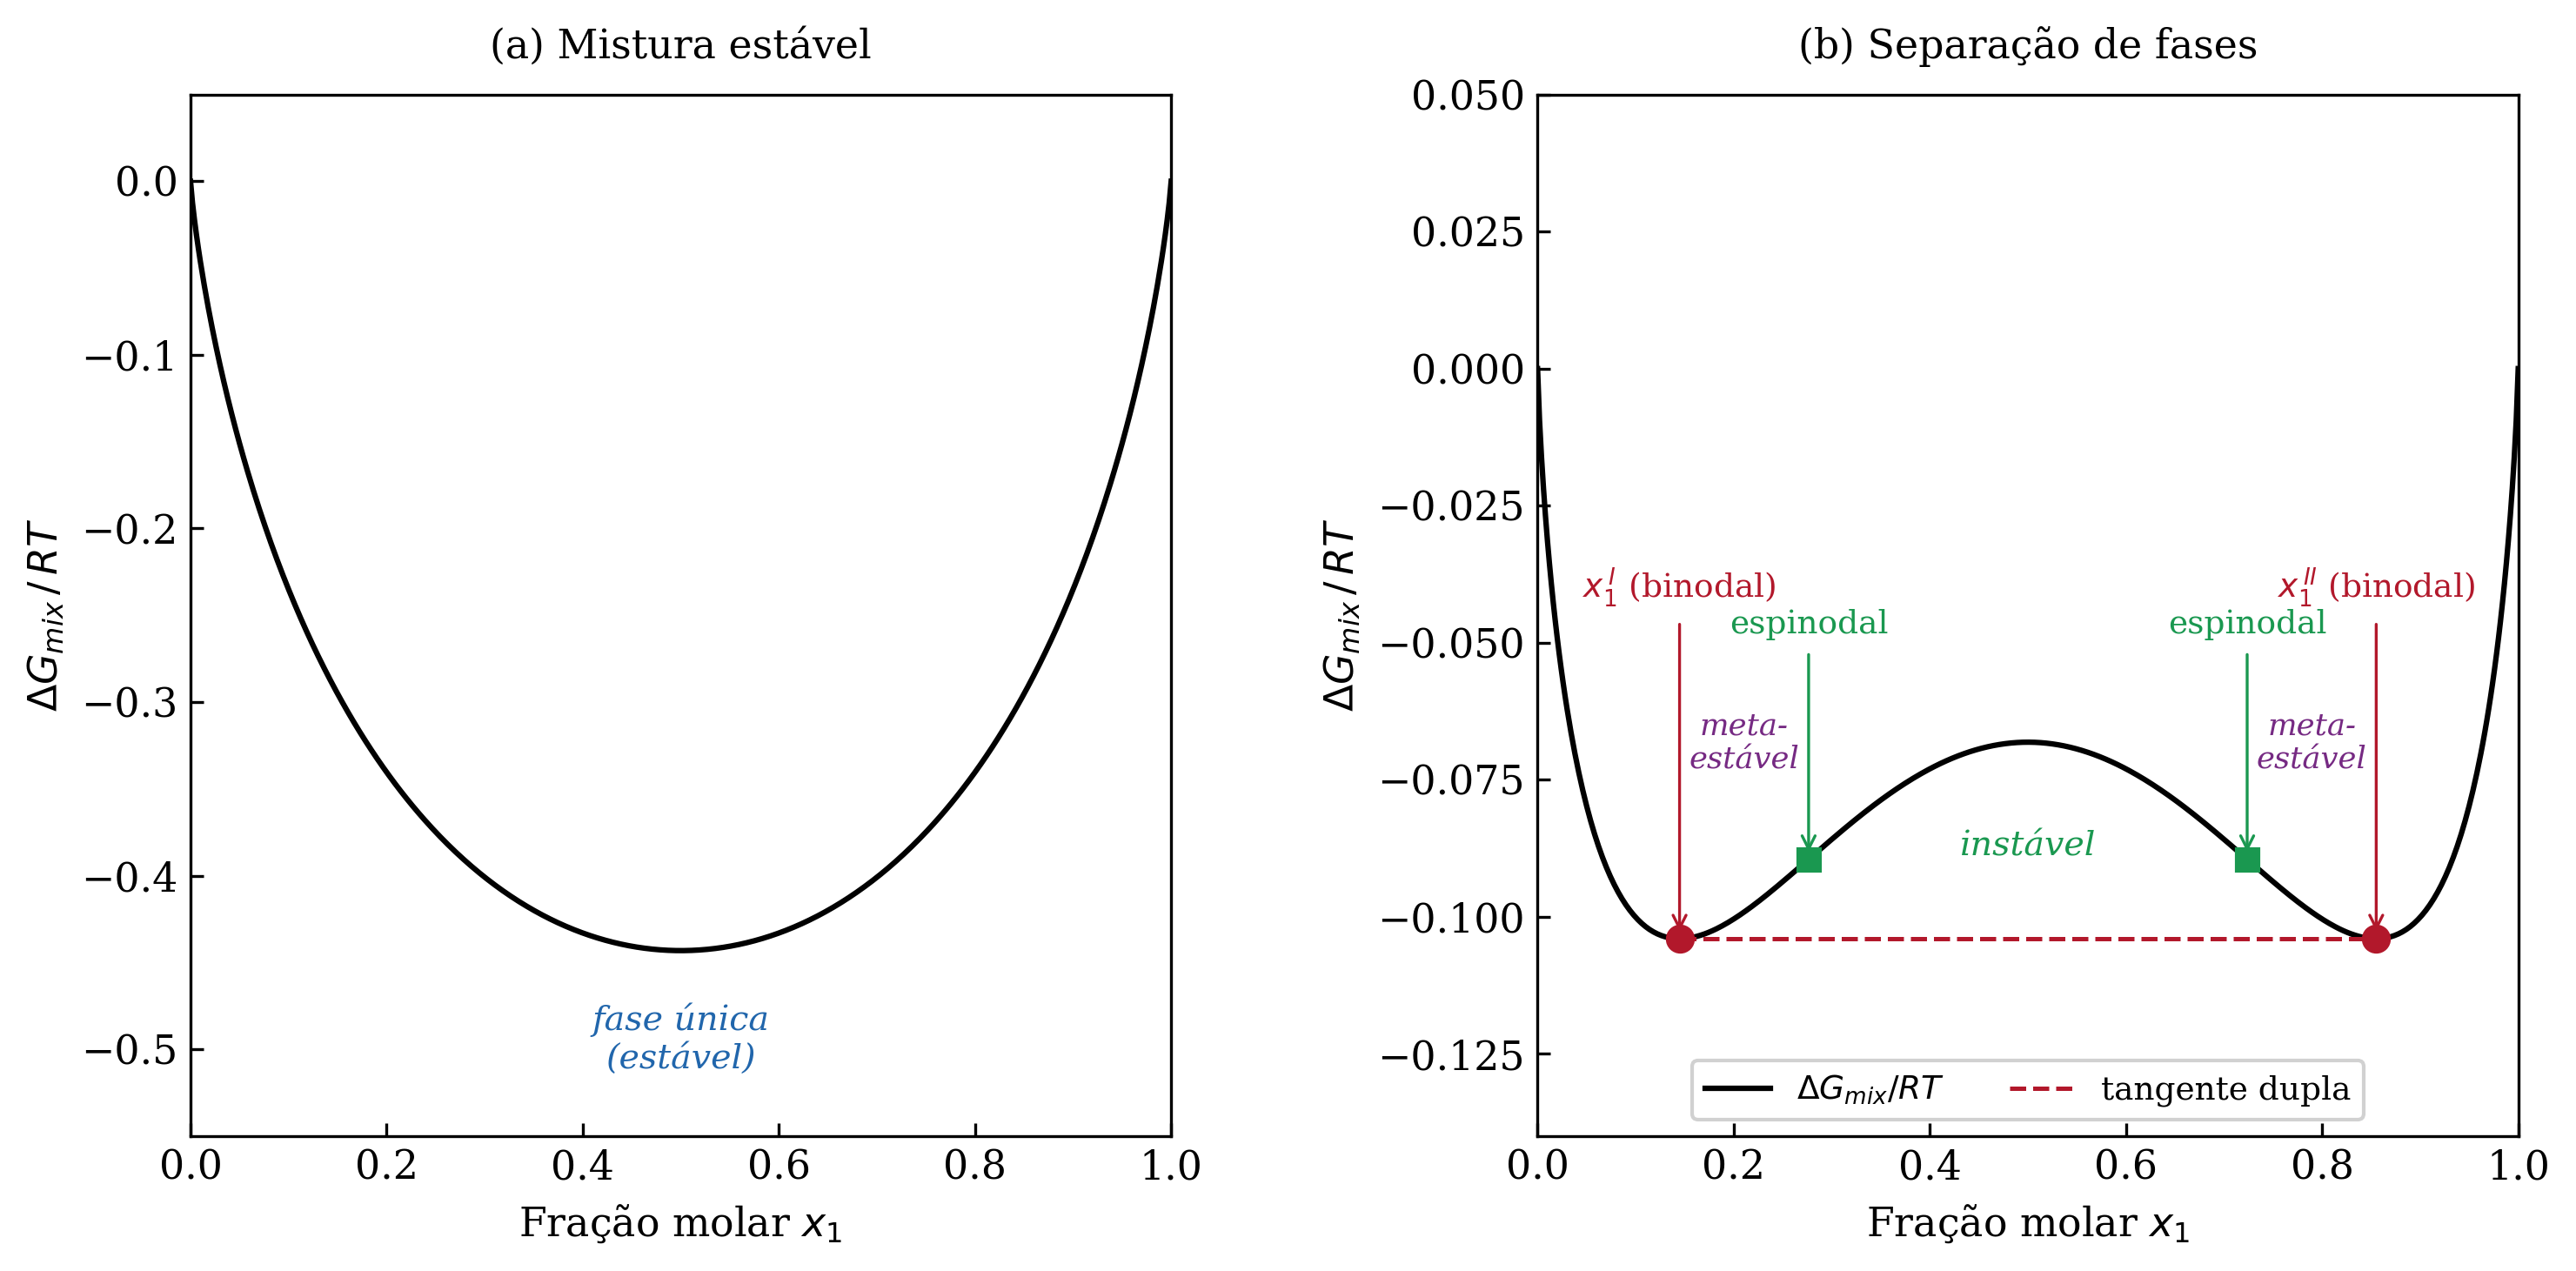
\includegraphics[width=1\linewidth]{imagens/fig1_gmix.png}
    \caption{\textit{Curva de $\Delta G_{mix}$ vs.\ composição para sistema binário, mostrando região estável, metaestável e instável, com pontos binodais e espinodais indicados.}}
    \label{fig:Curva_ΔGmix}
\end{figure}

Dessa análise decorrem duas fronteiras importantes. A curva \textit{binodal} é o lugar geométrico das composições em equilíbrio, determinadas pela tangente dupla, e delimita a região na qual o sistema se separa em duas fases. A curva \textit{espinodal}, definida pelos pontos de inflexão da curva de $\Delta G_{mix}$ (onde $\partial^2 \Delta G_{mix} / \partial x_i^2 = 0$), delimita a fronteira entre a região metaestável (entre a binodal e a espinodal, onde a mistura é localmente estável mas globalmente desfavorável) e a região instável (dentro da espinodal, onde qualquer flutuação infinitesimal de composição leva à separação espontânea). Na prática, tanto misturas metaestáveis quanto instáveis tendem a se separar, e as composições finais das fases são sempre dadas pela curva binodal\cite{smith2005}.

% -----------------------------------------------------------------
% Critério do plano tangente (TPD)
% -----------------------------------------------------------------

A construção geométrica da tangente dupla, descrita acima para o caso binário, generaliza-se para sistemas com três ou mais componentes por meio do critério do plano tangente (\textit{tangent plane distance}, TPD), formulado por \citeonline{baker1982} e sistematizado por \citeonline{michelsen1982}. Em vez de inspecionar visualmente a curvatura da superfície de energia de Gibbs, o critério TPD testa analiticamente se uma composição global $\mathbf{z}$ é estável, verificando se existe alguma composição de teste $\mathbf{x}$ capaz de reduzir a energia livre da mistura em relação ao plano tangente à superfície de $\Delta G_{mix}$ no ponto $\mathbf{z}$. A função de distância ao plano tangente é definida como\cite{michelsen1982}:

\begin{equation}
    TPD(\mathbf{x}) = \sum_{i} x_i
    \left[
        \ln(x_i \, \gamma_i(\mathbf{x})) - \ln(z_i \, \gamma_i(\mathbf{z}))
    \right]
    \label{eq:tpd}
\end{equation}

Se $TPD(\mathbf{x}) \geq 0$ para toda composição de teste $\mathbf{x}$ no espaço de composições, a mistura na composição $\mathbf{z}$ é estável como fase única. Se, ao contrário, existe algum $\mathbf{x}$ para o qual $TPD(\mathbf{x}) < 0$, a composição $\mathbf{z}$ é instável, e o sistema se separa espontaneamente em duas ou mais fases cujas composições minimizam a energia de Gibbs global\cite{michelsen1982}. Esse critério é o análogo multicomponente da condição de convexidade discutida para o caso binário (Equação~\ref{eq:gmix_total}), com a vantagem de ser diretamente aplicável a sistemas ternários como os estudados neste trabalho, nos quais a inspeção gráfica direta da superfície de $\Delta G_{mix}$ é pouco prática. A aplicação computacional do critério TPD aos sistemas ternários deste trabalho é detalhada no Capítulo~\ref{cap:metodologia}.

% -----------------------------------------------------------------
% Diagramas ternários
% -----------------------------------------------------------------

Para sistemas com três componentes, como os estudados neste trabalho, a representação do equilíbrio líquido-líquido é feita em diagramas ternários triangulares, nos quais cada vértice do triângulo equilátero corresponde a um componente puro e cada ponto no interior do triângulo representa uma composição da mistura ternária. A leitura das composições segue a convenção de que a fração molar (ou mássica) de cada componente é proporcional à distância perpendicular do ponto ao lado oposto ao vértice correspondente, de modo que a soma das três frações é sempre igual à unidade\cite{smith2005}.

\begin{figure}[H]
    \centering
    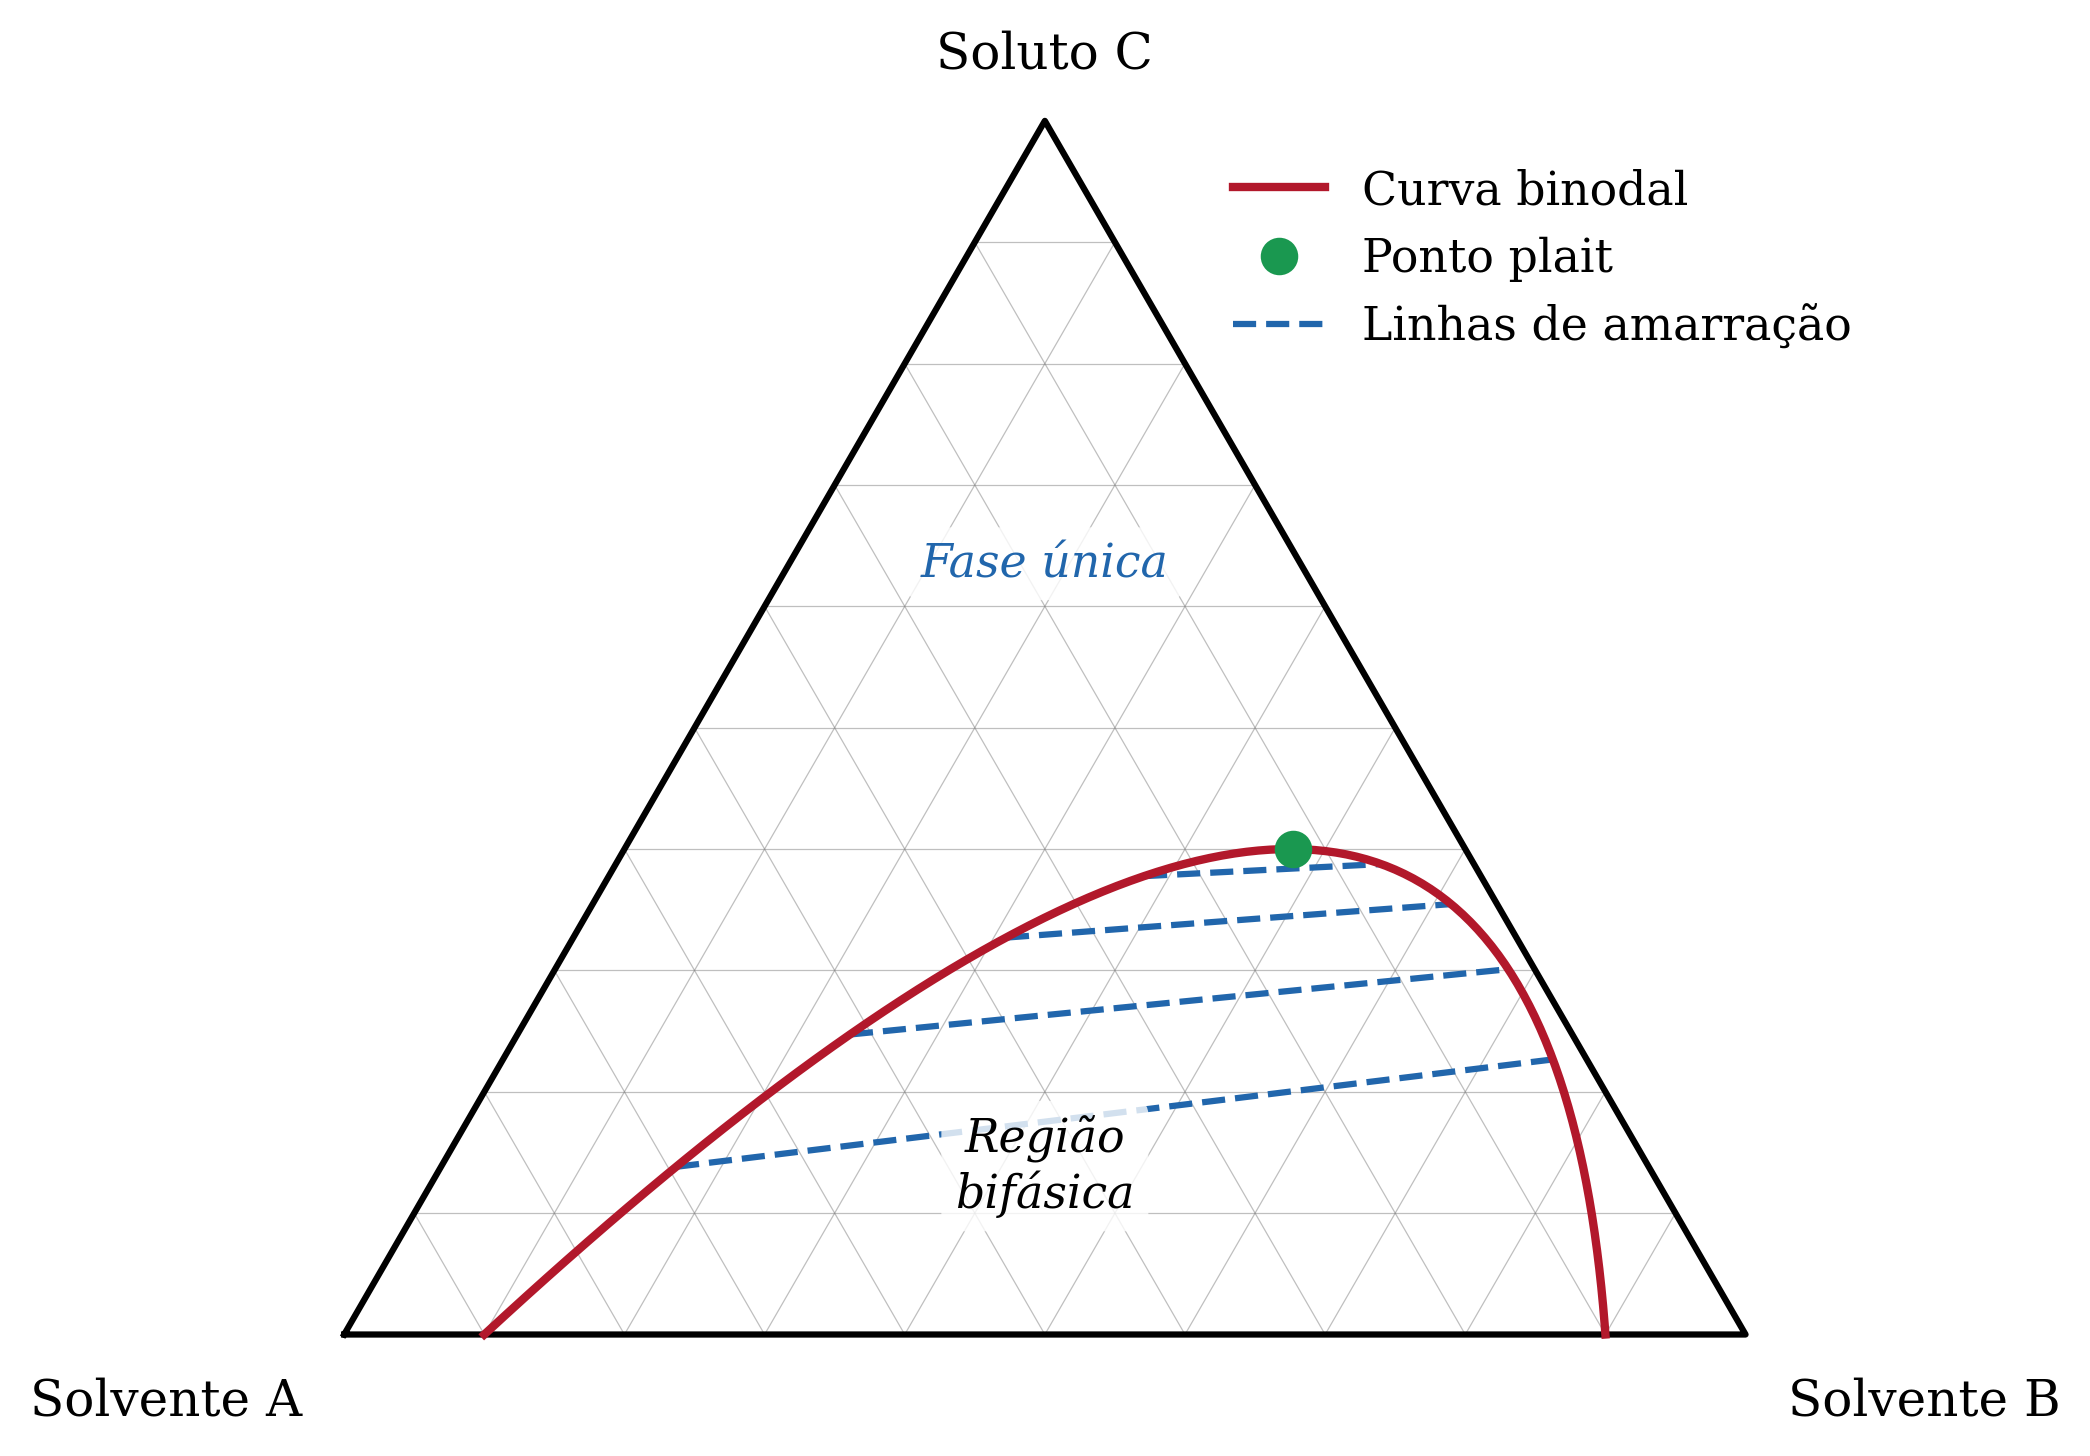
\includegraphics[width=0.8\linewidth]{imagens/fig2_diagrama_ternario.png}
    \caption{Diagrama ternário esquemático com curva binodal, linhas de amarração, ponto crítico de mistura e indicação das regiões monofásica e bifásica.}
    \label{fig:placeholder}
\end{figure}

No diagrama ternário, a região de duas fases é delimitada pela curva binodal (também denominada curva de solubilidade), que separa as composições em que o sistema existe como uma única fase líquida homogênea daquelas em que ocorre separação em duas fases. Uma composição global situada dentro da região bifásica se divide em duas fases cujas composições são dadas pelas extremidades da \textit{linha de amarração} (\textit{tie line}) que passa por aquele ponto. As linhas de amarração são segmentos de reta que conectam as composições das duas fases em equilíbrio, e sua inclinação e comprimento variam ao longo da curva binodal: à medida que se aproximam do ponto crítico de mistura (\textit{plait point}), as tie lines se tornam progressivamente mais curtas, até se reduzirem a um ponto no qual as composições e as propriedades das duas fases se tornam idênticas\cite{smith2005,treybal1980}.

Um aspecto relevante para a interpretação dos resultados deste trabalho é a relação entre a extensão da região bifásica e o efeito do cossolvente. Quando um terceiro componente (como o líquido iônico prótico) é adicionado ao sistema binário \{trioleína + etanol\}, a curva binodal se desloca, alterando a extensão da região de duas fases. Se o cossolvente aumenta a miscibilidade mútua dos reagentes, a região bifásica se contrai; se, ao contrário, o terceiro componente atua como agente de separação, a região bifásica se expande. A análise comparativa dos diagramas ternários simulados para os sistemas contendo [2-HEA][Hx] e [DETA][Hx], objetivo deste trabalho, permite avaliar quantitativamente se os LIPs são eficazes em promover a miscibilidade do sistema reacional.

As linhas de amarração fornecem ainda uma informação complementar de interesse prático: a razão de distribuição do cossolvente entre as fases. A partir das composições nas extremidades de cada tie line, pode-se calcular o coeficiente de distribuição $K_i = x_i^{II} / x_i^{I}$ de cada componente, que indica a afinidade preferencial da espécie por uma das fases\cite{treybal1980}. Para a avaliação do efeito cossolvente, a análise conjunta das tie lines e do coeficiente de distribuição do LIP permite verificar se o cossolvente se distribui entre ambas as fases ou se concentra preferencialmente em uma delas.

\section{O modelo de solvatação COSMO}
\label{sec:cosmo_solvatacao}

Os modelos da família COSMO (\textit{COnductor-like Screening MOdel}) partem de uma premissa comum: as interações intermoleculares em fase líquida podem ser descritas a partir das propriedades eletrostáticas da superfície molecular de cada espécie, calculadas individualmente por métodos de química quântica. O ponto de partida é o modelo de solvatação proposto por \citeonline{klamt1993}, posteriormente refinado por \citeonline{klamt1995}, no qual cada molécula é tratada como se estivesse imersa em um condutor perfeito. Esta seção apresenta os fundamentos desse cálculo, que constitui a etapa de entrada para o modelo COSMO-SAC discutido na Seção\ref{sec:cosmosac}.

% -----------------------------------------------------------------
% A cavidade COSMO e as cargas de blindagem
% -----------------------------------------------------------------

No modelo COSMO, a molécula de interesse é inserida em uma cavidade construída a partir dos raios de van der Waals dos átomos que a compõem. O espaço exterior à cavidade é preenchido por um condutor ideal, cuja constante dielétrica é infinita\cite{klamt1993}. Essa escolha é deliberada: em um condutor perfeito, o campo elétrico externo à cavidade é nulo, o que significa que a distribuição de cargas da molécula induz, na superfície interna da cavidade, um conjunto de cargas de blindagem (\textit{screening charges}) que cancelam exatamente o potencial eletrostático gerado pela molécula no exterior. A determinação dessas cargas de blindagem é realizada por meio de um cálculo autoconsistente de química quântica, tipicamente no formalismo da teoria do funcional da densidade (DFT), no qual a estrutura eletrônica da molécula e as cargas de blindagem na superfície são otimizadas simultaneamente até a convergência\cite{klamt1995}.

\begin{figure}[H]
    \centering
    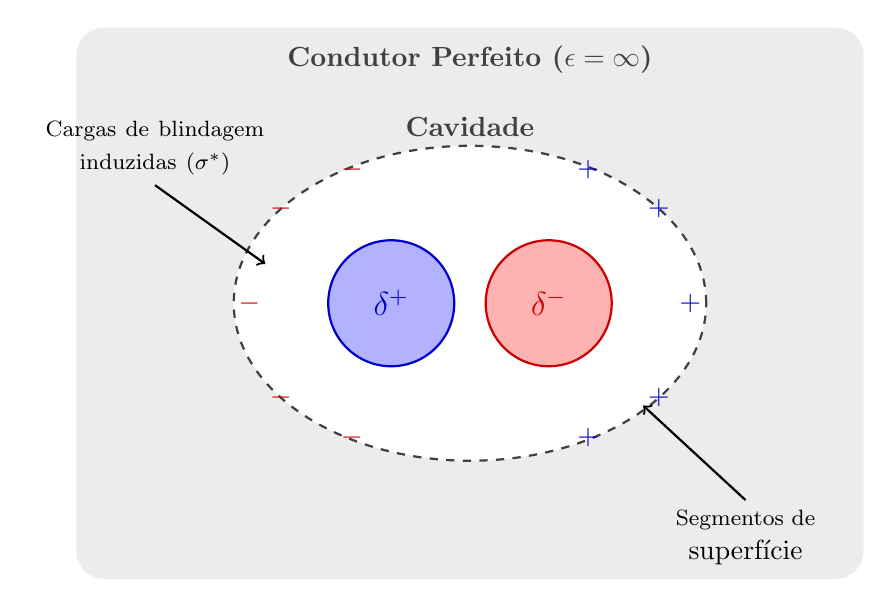
\begin{tikzpicture}
        
        % 1. Fundo representando o condutor perfeito
        % Uma caixa cinza com bordas arredondadas
        \fill[gray!15, rounded corners=10pt] (-5,-3.5) rectangle (5,3.5);
        \node[above, darkgray] at (0, 2.8) {\textbf{Condutor Perfeito ($\epsilon = \infty$)}};

        % 2. A Cavidade COSMO
        % Desenhada como uma elipse branca com borda tracejada
        \fill[white] (0,0) ellipse (3cm and 2cm);
        \draw[thick, dashed, darkgray] (0,0) ellipse (3cm and 2cm);
        
        % Label da cavidade
        \node[above, darkgray] at (0, 2) {\textbf{Cavidade}};

        % 3. Molécula Genérica (Dipolo)
        % Átomo com carga parcial positiva (Azul)
        \fill[blue!30] (-1,0) circle (0.8cm);
        \draw[thick, blue!80!black] (-1,0) circle (0.8cm);
        \node[blue!80!black] at (-1, 0) {\large $\delta^+$};
        
        % Átomo com carga parcial negativa (Vermelho)
        \fill[red!30] (1,0) circle (0.8cm);
        \draw[thick, red!80!black] (1,0) circle (0.8cm);
        \node[red!80!black] at (1, 0) {\large $\delta^-$};

        % 4. Segmentos de Superfície e Cargas de Triagem (\sigma)
        % Cargas negativas induzidas próximas ao polo positivo da molécula
        \node[red!80!black, font=\bfseries] at (-2.8, 0) {$-$};
        \node[red!80!black, font=\bfseries] at (-2.4, 1.2) {$-$};
        \node[red!80!black, font=\bfseries] at (-2.4, -1.2) {$-$};
        \node[red!80!black, font=\bfseries] at (-1.5, 1.7) {$-$};
        \node[red!80!black, font=\bfseries] at (-1.5, -1.7) {$-$};

        % Cargas positivas induzidas próximas ao polo negativo da molécula
        \node[blue!80!black, font=\bfseries] at (2.8, 0) {$+$};
        \node[blue!80!black, font=\bfseries] at (2.4, 1.2) {$+$};
        \node[blue!80!black, font=\bfseries] at (2.4, -1.2) {$+$};
        \node[blue!80!black, font=\bfseries] at (1.5, 1.7) {$+$};
        \node[blue!80!black, font=\bfseries] at (1.5, -1.7) {$+$};

        % 5. Setas e Rótulos Explicativos
        % Seta apontando para as cargas de triagem
        \draw[<-, thick] (-2.6, 0.5) -- (-4, 1.5) 
            node[above, align=center, text width=3cm] {\footnotesize Cargas de blindagem induzidas ($\sigma^*$)};
            
        % Seta apontando para a fronteira (segmentos)
        \draw[<-, thick] (2.2, -1.3) -- (3.5, -2.5) 
            node[below, align=center] {\footnotesize Segmentos de\\superfície};

    \end{tikzpicture}
    \vspace{0.5cm}
    \caption{Representação esquemática do modelo COSMO mostrando
    a molécula na cavidade, o condutor perfeito e os segmentos de
    superfície com suas cargas de blindagem. Adaptado de Lin e Sandler (2002).}
    \label{fig:cosmo_cavity}
\end{figure}

O resultado do cálculo COSMO é uma superfície molecular discretizada em $n$ segmentos, cada um caracterizado por uma área $a_n$ e uma densidade de carga de blindagem $\sigma_n^{*}$ (em unidades de carga por unidade de área, tipicamente e/\AA$^2$). Essa distribuição de cargas na superfície reflete, de forma compacta, toda a informação relevante sobre a capacidade da molécula de interagir eletrostaticamente com o meio ao seu redor: regiões da superfície com $\sigma > 0$ correspondem a segmentos onde a molécula apresenta carga negativa exposta (e o condutor responde com carga positiva de blindagem), enquanto regiões com $\sigma < 0$ indicam carga positiva na superfície molecular. Segmentos com $\sigma \approx 0$ correspondem a regiões apolares da molécula\cite{lin2002}. 
% -----------------------------------------------------------------
% Do condutor perfeito ao solvente real
% -----------------------------------------------------------------

Uma observação importante é que o cálculo COSMO descreve a molécula em um condutor perfeito, e não em um solvente real. A transição do condutor ideal para um meio dielétrico finito (como um líquido) requer uma correção, que nos modelos da família COSMO é feita por meio de um fator de escala aplicado às cargas de blindagem\cite{klamt1995}. Essa correção, embora conceitualmente relevante, não altera a estrutura do cálculo: o procedimento continua sendo resolver a equação de Schrödinger-Kohn-Sham na presença do contínuo dielétrico e extrair as cargas de superfície. Os detalhes do nível de teoria empregado (funcional DFT e conjunto de funções de base), que influenciam a qualidade das cargas obtidas, são discutidos no Capítulo\ref{cap:metodologia} no contexto específico dos compostos estudados neste trabalho.

% -----------------------------------------------------------------
% Perfis de densidade de carga superficial (σ-profiles)
% -----------------------------------------------------------------

A representação tridimensional das cargas de blindagem sobre a superfície molecular (denominada $\sigma$-\textit{surface}) contém toda a informação necessária, porém não é diretamente utilizável nos cálculos de equilíbrio de fases, que requerem uma descrição estatística das interações entre segmentos. Para viabilizar essa descrição, a distribuição de cargas é projetada em um histograma unidimensional denominado \textit{perfil de densidade de carga superficial}, ou $\sigma$-\textit{profile}, designado por $p_i(\sigma)$\cite{lin2002}. O $\sigma$-profile de uma substância $i$ representa a distribuição de área superficial da molécula em função da densidade de carga $\sigma$:

\begin{equation}
    p_i(\sigma) = \frac{A_i(\sigma)}{A_i}
    \label{eq:sigma_profile}
\end{equation}

\noindent em que $A_i(\sigma)$ é a área total dos segmentos que possuem densidade de carga $\sigma$ e $A_i$ é a área total da cavidade da molécula $i$.

Antes de construir o histograma, contudo, as cargas brutas provenientes do cálculo COSMO ($\sigma_n^{*}$) passam por um procedimento de suavização (\textit{averaging}), no qual a carga de cada segmento é recalculada como uma média ponderada das cargas dos segmentos vizinhos. Essa etapa é necessária porque o modelo COSMO-SAC assume que todos os segmentos possuem a mesma área efetiva $a_{eff}$, e a suavização garante que a distribuição de cargas seja consistente com essa premissa\cite{lin2002}. O raio de suavização $r_{eff}$ é um dos parâmetros universais do modelo.

\begin{figure}[H]
    \centering
    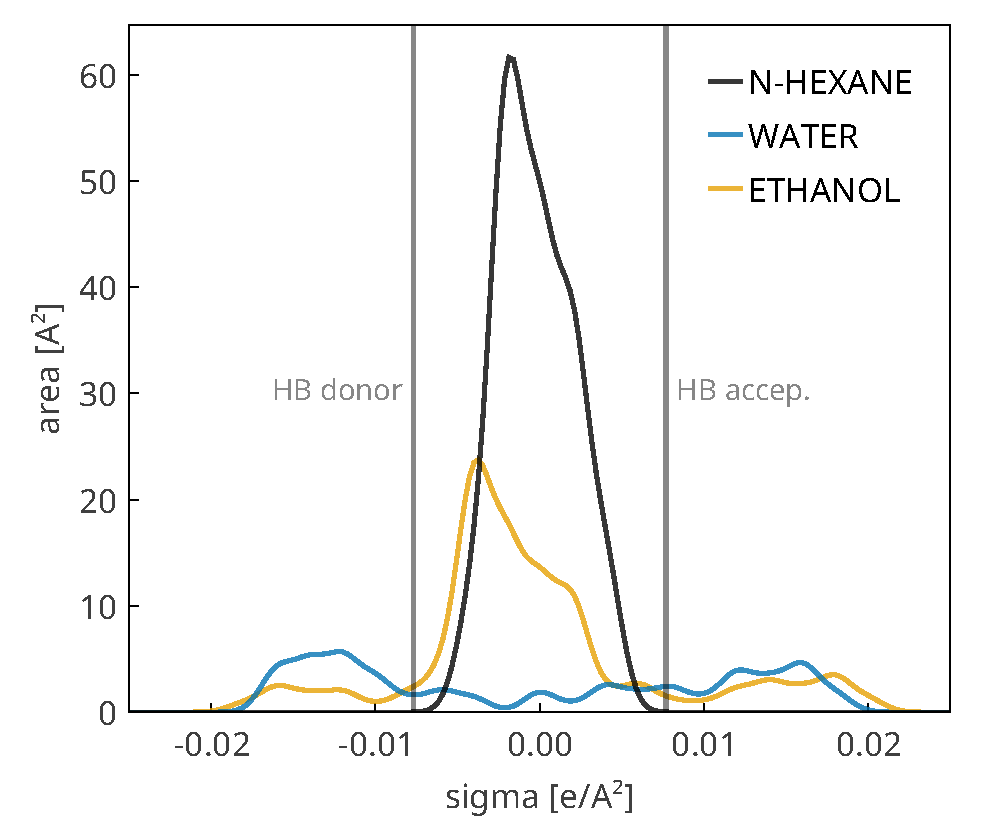
\includegraphics[width=0.5\textwidth]{imagens/N-HEXANE-WATER-ETHANOL.pdf}
    \caption{$\sigma$-\textit{profiles} de n-hexano, água e etanol, gerados no JCOSMO com a base GAMESS. As linhas verticais delimitam as regiões de doação (HB \textit{donor},  $\sigma < -0{,}0082$ e/\AA$^2$) e aceitação (HB \textit{accep.}, $\sigma > +0{,}0082$ e/\AA$^2$) de ligações de hidrogênio. A região central ($|\sigma| < 0{,}0082$ e/\AA$^2$) corresponde a segmentos apolares.
    Fonte: gerado no \textit{software} JCOSMO.}
    \label{fig:sigma_profiles}
\end{figure}
A interpretação física do $\sigma$-profile é direta e constitui uma das vantagens conceituais dos modelos baseados em COSMO. A região central do perfil ($\sigma \approx 0$) corresponde à área apolar da molécula, que interage com o meio apenas por forças de dispersão fracas. As regiões com $\sigma$ fortemente positivo (tipicamente $\sigma > +0{,}01$ e/\AA$^2$) correspondem a segmentos com carga negativa exposta na superfície molecular, como os pares de elétrons não ligantes de átomos de oxigênio ou nitrogênio, que são aceptores de ligações de hidrogênio. Simetricamente, as regiões com $\sigma$ fortemente negativo ($\sigma < -0{,}01$ e/\AA$^2$) correspondem a segmentos com carga positiva exposta, como os hidrogênios ligados a átomos eletronegativos, que são doadores de ligações de hidrogênio\cite{lin2002}. Dessa forma, uma molécula apolar como o hexano apresenta um $\sigma$-profile concentrado em torno de $\sigma = 0$, enquanto uma molécula como a água apresenta dois picos pronunciados nas regiões de doação e aceitação de hidrogênio. O etanol, por possuir tanto uma cadeia alquílica apolar quanto um grupo hidroxila, exibe um perfil intermediário com contribuições nas três regiões\cite{lin2002}.

Essa representação será particularmente útil na discussão dos resultados (Capítulo\ref{cap:resultados}), pois a comparação dos $\sigma$-profiles dos cátions [2-HEA]$^+$ e [DETA]$^+$ e do ânion [Hx]$^-$ permite identificar, em termos moleculares, as diferenças de interação que explicam o comportamento distinto dos dois LIPs como cossolventes no sistema \{trioleína + etanol\}.

\section{O modelo COSMO-SAC}
\label{sec:cosmosac}

O modelo COSMO-SAC (\textit{COnductor-like Screening MOdel -- Segment Activity Coefficient}) foi proposto por \citeonline{lin2002} como uma variação do modelo COSMO-RS (\textit{COSMO for Real Solvents}),  introduzido por \citeonline{klamt1995}. Ambos os modelos compartilham a premissa de que as interações intermoleculares em fase líquida podem ser calculadas a partir dos $\sigma$-profiles das espécies puras, sem necessidade de parâmetros ajustados a dados experimentais de misturas. A diferença reside na formulação termodinâmica empregada: enquanto o COSMO-RS utiliza uma expressão analítica direta para o potencial químico dos segmentos, o COSMO-SAC reformula o problema em termos de coeficientes de atividade de segmento, dentro de um arcabouço compatível com os modelos clássicos de $G^E$ utilizados em engenharia química\cite{lin2002,gerber2010}.

% -----------------------------------------------------------------
% Estrutura geral do coeficiente de atividade
% -----------------------------------------------------------------

No COSMO-SAC, o coeficiente de atividade do componente $i$ em uma solução $S$ é expresso como a soma de duas contribuições\cite{lin2002}:

\begin{equation}
    \ln \gamma_i = \ln \gamma_i^{comb} + \ln \gamma_i^{res}
    \label{eq:gamma_cosmo}
\end{equation}

A contribuição residual ($\ln \gamma_i^{res}$) captura os efeitos das interações eletrostáticas e de ligações de hidrogênio entre os segmentos de superfície, e é calculada a partir dos $\sigma$-profiles. A contribuição combinatorial ($\ln \gamma_i^{comb}$) descreve os efeitos entrópicos associados às diferenças de tamanho e forma entre as moléculas da mistura, e é calculada a partir do volume e da área da cavidade COSMO de cada espécie. As duas contribuições são apresentadas a seguir.

% -----------------------------------------------------------------
% Contribuição residual
% -----------------------------------------------------------------

\subsection{Contribuição residual: interações entre segmentos de
superfície}
\label{subsec:cosmo_residual}

A contribuição residual ao coeficiente de atividade é obtida a partir da diferença entre a energia livre de restauração (\textit{restoring free energy}) do soluto $i$ na mistura $S$ e no líquido puro\cite{lin2002}:

\begin{equation}
    \ln \gamma_i^{res} =
    \frac{\Delta G_i^{*res/S} - \Delta G_i^{*res/i}}{RT}
    \label{eq:gamma_residual}
\end{equation}

A energia livre de restauração representa o custo energético de ``religar'' as interações eletrostáticas da molécula quando ela é transferida do condutor perfeito (onde as cargas estão perfeitamente blindadas) para o meio líquido real (onde a blindagem é imperfeita)\cite{lin2002}. A diferença entre os dois termos na Equação\ref{eq:gamma_residual} garante que, quando o soluto se encontra em seu próprio líquido puro, $\ln \gamma_i^{res} = 0$, como esperado. A energia livre de restauração é calculada como uma soma sobre todos os segmentos da molécula $i$, ponderada pelo $\sigma$-profile da espécie e pelo coeficiente de atividade de cada tipo de segmento\cite{lin2002}:

\begin{equation}
    \frac{\Delta G_i^{*res/S}}{RT} =
    n_i \sum_{\sigma_m} p_i(\sigma_m) \, \ln \Gamma_S(\sigma_m)
    \label{eq:energia_restauracao}
\end{equation}

\noindent em que $n_i = A_i / a_{eff}$ é o número total de segmentos na superfície da molécula $i$, $p_i(\sigma_m)$ é o $\sigma$-profile da espécie pura $i$ e $\Gamma_S(\sigma_m)$ é o coeficiente de atividade do segmento com carga $\sigma_m$ na mistura $S$.

O coeficiente de atividade de segmento $\Gamma_S(\sigma_m)$ é o elemento central do modelo. Ele mede o quanto um segmento de carga $\sigma_m$ se desvia do comportamento ideal na mistura, e é obtido pela solução da seguinte equação implícita\cite{lin2002}:

\begin{equation}
    \ln \Gamma_S(\sigma_m) =
    -\ln \left\{
        \sum_{\sigma_n} p_S(\sigma_n) \, \Gamma_S(\sigma_n)
        \exp \left[
            -\frac{\Delta W(\sigma_m, \sigma_n)}{RT}
        \right]
    \right\}
    \label{eq:gamma_segmento}
\end{equation}

\noindent em que $p_S(\sigma_n)$ é o $\sigma$-profile da mistura $S$ e $\Delta W(\sigma_m, \sigma_n)$ é a energia de interação entre um par de segmentos com cargas $\sigma_m$ e $\sigma_n$. A Equação\ref{eq:gamma_segmento} é implícita porque $\Gamma_S(\sigma_m)$
aparece em ambos os lados, e deve ser resolvida iterativamente até a convergência\cite{lin2002}.

O $\sigma$-profile da mistura é construído como a média ponderada dos $\sigma$-profiles dos componentes puros, utilizando as frações molares como pesos\cite{lin2002}:

\begin{equation}
    p_S(\sigma) = \sum_{i=1}^{c} x_i \, p_i(\sigma)
    \label{eq:sigma_profile_mistura}
\end{equation}

Essa expressão reflete uma das hipóteses centrais do modelo: os segmentos de superfície são tratados como independentes e a composição da ``superfície da mistura'' é simplesmente a soma das superfícies de cada componente, ponderada pela composição\cite{lin2002}.

% -----------------------------------------------------------------
% Energia de interação entre segmentos
% -----------------------------------------------------------------

\subsection{Energia de interação entre segmentos}
\label{subsec:cosmo_interacao}

A energia de interação entre dois segmentos de superfície com densidades de carga $\sigma_m$ e $\sigma_n$ é composta por duas contribuições\cite{lin2002}:

\begin{equation}
    \Delta W(\sigma_m, \sigma_n) =
    \Delta W_{mf}(\sigma_m, \sigma_n)
    + \Delta W_{hb}(\sigma_m, \sigma_n)
    \label{eq:energia_interacao}
\end{equation}

A primeira contribuição é a energia de \textit{misfit} (desajuste eletrostático), que penaliza o contato entre segmentos cujas cargas de blindagem não se cancelam mutuamente:

\begin{equation}
    \Delta W_{mf}(\sigma_m, \sigma_n) =
    \frac{R'}{2} (\sigma_m + \sigma_n)^2
    \label{eq:energia_misfit}
\end{equation}

\noindent em que $R'$ é uma constante que depende do fator de polarização $f_{pol}$ e da área efetiva de segmento $a_{eff}$. O termo $(\sigma_m + \sigma_n)^2$ tem um significado físico intuitivo: quando dois segmentos com cargas opostas entram em contato ($\sigma_m + \sigma_n \approx 0$), a energia de misfit é mínima, pois as cargas se cancelam mutuamente, assim como ocorreria no condutor perfeito. Quando dois segmentos de mesma carga se encontram, a soma é grande e a penalidade energética é máxima, refletindo a situação desfavorável em que a blindagem é deficiente\cite{lin2002}.

A segunda contribuição é a energia de ligação de hidrogênio, que estabiliza o contato entre segmentos doadores e aceptores de ligações de hidrogênio\cite{lin2002}:

\begin{equation}
    \Delta W_{hb}(\sigma_m, \sigma_n) =
    c_{hb} \,
    \max\!\left[0, \;\sigma_{acc} - \sigma_{hb}\right]
    \cdot
    \min\!\left[0, \;\sigma_{don} + \sigma_{hb}\right]
    \label{eq:energia_hbond}
\end{equation}

\noindent em que $c_{hb}$ é a constante de ligação de hidrogênio, $\sigma_{hb}$ é o valor de corte que define quais segmentos são capazes de participar de ligações de hidrogênio, e $\sigma_{acc}$ e $\sigma_{don}$ são, respectivamente, o maior e o menor valor entre $\sigma_m$ e $\sigma_n$. A Equação\ref{eq:energia_hbond} é construída de modo que a contribuição de ligação de hidrogênio seja não nula apenas quando um segmento fortemente positivo ($\sigma_{acc} > \sigma_{hb}$, aceptor) interage com um segmento fortemente negativo ($\sigma_{don} < -\sigma_{hb}$, doador). Nesse caso, o produto é negativo, reduzindo a energia total de interação e estabilizando o contato\cite{lin2002}. Para pares de segmentos que não satisfazem o critério de corte, a contribuição de ligação de hidrogênio é nula.

% -----------------------------------------------------------------
% Extensão HB2: subdivisão da superfície de ligação de hidrogênio
% -----------------------------------------------------------------

A formulação original de \citeonline{lin2002}, apresentada na Equação~\ref{eq:energia_hbond}, trata toda a superfície capaz de participar de ligações de hidrogênio de forma homogênea, com uma única constante $c_{hb}$ e um único valor de corte $\sigma_{hb}$. \citeonline{hsieh2010} propuseram um refinamento desse tratamento, denominado COSMO-SAC-HB2 (ou COSMO-SAC-2010), no qual os segmentos de superfície capazes de participar de ligações de hidrogênio são subdivididos em dois tipos: segmentos associados a grupos hidroxila (tipo OH) e segmentos associados a outros grupos doadores ou aceptores de hidrogênio, como nitrogênio, oxigênio não hidroxílico e flúor (tipo OT). Essa subdivisão reflete a observação empírica de que a intensidade da ligação de hidrogênio varia conforme o tipo químico do grupo envolvido, e não apenas conforme a magnitude da densidade de carga do segmento.

Na prática, essa subdivisão se propaga por todo o formalismo do COSMO-SAC: o $\sigma$-profile de cada espécie pura, antes descrito por uma única distribuição $p_i(\sigma)$ (Equação~\ref{eq:sigma_profile}), passa a ser decomposto em três distribuições parciais,
\begin{equation}
    p_i(\sigma) = p_i^{nhb}(\sigma) + p_i^{OH}(\sigma) + p_i^{OT}(\sigma),
    \label{eq:sigma_profile_hb2}
\end{equation}
correspondentes, respectivamente, aos segmentos sem capacidade de ligação de hidrogênio, aos segmentos do tipo OH e aos segmentos do tipo OT. A energia de interação entre dois segmentos (Equação~\ref{eq:energia_hbond}) passa a depender não apenas das densidades de carga $\sigma_m$ e $\sigma_n$, mas também dos tipos $t_m, t_n \in \{OH, OT\}$ de cada segmento, por meio de uma constante de ligação de hidrogênio específica para cada combinação de tipos:
\begin{equation}
    \Delta W_{hb}(\sigma_m, \sigma_n) =
    c_{hb}^{(t_m, t_n)} \,
    \max\!\left[0, \;\sigma_{acc} - \sigma_{hb}\right]
    \cdot
    \min\!\left[0, \;\sigma_{don} + \sigma_{hb}\right],
    \label{eq:energia_hbond_hb2}
\end{equation}
em que $c_{hb}^{(OH,OH)}$, $c_{hb}^{(OT,OT)}$ e $c_{hb}^{(OH,OT)}$ são três constantes distintas, ajustadas por \citeonline{hsieh2010} a um banco de dados experimental de equilíbrio de fases mais amplo do que o utilizado na parametrização original de \citeonline{lin2002}. O valor de corte $\sigma_{hb}$ permanece único, comum aos dois tipos de segmento. Essa subdivisão permite, por exemplo, que a interação entre dois segmentos hidroxila (como em uma ligação O–H\textperiodcentered\textperiodcentered\textperiodcentered O entre duas moléculas de álcool) seja tratada com uma intensidade diferente da interação entre um segmento hidroxila e um segmento amino (como ocorre entre o álcool e o líquido iônico prótico nos sistemas estudados neste trabalho, Seção~\ref{subsec:ligacao_hidrogenio}), refinamento particularmente relevante para a diversidade de grupos doadores e aceptores de hidrogênio presentes nos sistemas \{triglicerídeo + álcool + líquido iônico prótico\} deste trabalho. A parametrização COSMO-SAC-HB2 é a efetivamente empregada nos cálculos deste trabalho (Capítulo~\ref{cap:metodologia}), e as demais equações do modelo (contribuição combinatorial, energia de misfit) permanecem inalteradas em relação à formulação original.

% -----------------------------------------------------------------
% Contribuição combinatorial
% -----------------------------------------------------------------

\subsection{Contribuição combinatorial: efeitos de tamanho e forma}
\label{subsec:cosmo_combinatorial}

A contribuição combinatorial ao coeficiente de atividade é calculada pelo modelo de Staverman-Guggenheim, que descreve os efeitos entrópicos decorrentes das diferenças de tamanho e forma entre as moléculas da mistura\cite{lin2002}:

\begin{equation}
    \ln \gamma_i^{comb} =
    \ln \frac{\phi_i}{x_i}
    + \frac{z}{2} \, q_i \, \ln \frac{\theta_i}{\phi_i}
    + l_i
    - \frac{\phi_i}{x_i} \sum_{j} x_j \, l_j
    \label{eq:gamma_combinatorial}
\end{equation}

\noindent em que $z = 10$ é o número de coordenação da rede, $\phi_i = r_i x_i / \sum_j r_j x_j$ é a fração volumétrica normalizada, $\theta_i = q_i x_i / \sum_j q_j x_j$ é a fração de área superficial normalizada, e $l_i = (z/2)(r_i - q_i) - (r_i - 1)$. Os parâmetros $r_i$ e $q_i$ são, respectivamente, o volume e a área superficial normalizados da molécula $i$, obtidos diretamente da cavidade COSMO\cite{lin2002}:

\begin{equation}
    r_i = \frac{V_i}{r_{std}} \qquad \text{e} \qquad
    q_i = \frac{A_i}{q_{std}}
    \label{eq:ri_qi}
\end{equation}

\noindent em que $V_i$ e $A_i$ são o volume e a área total da cavidade COSMO da molécula $i$, e $r_{std}$ e $q_{std}$ são parâmetros universais de normalização. A contribuição combinatorial tende a ser mais significativa em misturas de moléculas com tamanhos muito diferentes, como é o caso do sistema \{trioleína + etanol\}, em que a trioleína (\ce{C57H104O6}, massa molar 885,4g/mol) é consideravelmente maior que o etanol (\ce{C2H6O}, massa molar 46,1g/mol).

% -----------------------------------------------------------------
% Parâmetros universais
% -----------------------------------------------------------------

\subsection{Parâmetros universais do modelo}
\label{subsec:cosmo_parametros}

Um aspecto importante do COSMO-SAC é que o modelo depende de um conjunto reduzido de parâmetros universais, que são ajustados uma única vez a partir de um banco de dados de propriedades termodinâmicas e permanecem fixos para qualquer sistema subsequente. Os principais parâmetros são a área efetiva de segmento $a_{eff}$ (que define o tamanho dos segmentos no procedimento de suavização), o raio de suavização $r_{eff}$, o fator de polarização $f_{pol}$, a constante de ligação de hidrogênio $c_{hb}$, o valor de corte $\sigma_{hb}$ e os parâmetros de normalização $r_{std}$ e $q_{std}$\cite{lin2002,gerber2010}. Os valores numéricos desses parâmetros dependem do nível de teoria utilizado na geração dos $\sigma$-profiles (isto é, do pacote de química quântica empregado), e diferentes parametrizações foram propostas na literatura para $\sigma$-profiles gerados com DMol3, GAMESS, MOPAC e TURBOMOLE\cite{gerber2010}. A consistência entre o nível de teoria dos cálculos COSMO e a parametrização do modelo é essencial para a qualidade das predições, como discutido por
\citeonline{gerber2010}, e constitui um aspecto central da metodologia adotada neste trabalho (Capítulo\ref{cap:metodologia}).

O fato de esses parâmetros serem universais (isto é, não específicos para cada sistema ou mistura) é o que confere ao COSMO-SAC sua natureza preditiva \textit{a priori}: uma vez calibrado o modelo com uma base de dados de referência, qualquer sistema pode ser tratado desde que os $\sigma$-profiles dos componentes estejam disponíveis. Não há necessidade de parâmetros binários de interação ajustados a dados experimentais da mistura de interesse, ao contrário do que ocorre nos modelos de contribuição por grupos como o UNIFAC-LL, discutido na Seção\ref{sec:unifacll}.

\section{Tratamento de líquidos iônicos no formalismo COSMO}
\label{sec:cosmo_li}

O modelo COSMO-SAC, tal como formulado por \citeonline{lin2002}, foi desenvolvido e parametrizado para misturas de moléculas neutras. A aplicação do modelo a sistemas contendo líquidos iônicos introduz uma dificuldade conceitual que não se apresenta para compostos moleculares convencionais: o LI é composto por dois íons (cátion e ânion), e a forma como essas espécies são representadas no cálculo COSMO afeta diretamente os $\sigma$-profiles gerados e, consequentemente, a qualidade das predições de equilíbrio de fases. Duas estratégias principais foram propostas na literatura para lidar com essa questão, denominadas abordagem CA (par iônico) e abordagem C+A (íons separados)\cite{dominguez2014}.

% -----------------------------------------------------------------
% Abordagem CA: par iônico neutro
% -----------------------------------------------------------------

Na abordagem CA, o cátion e o ânion são tratados como uma única entidade neutra. O cálculo COSMO é realizado sobre o par iônico, gerando um único $\sigma$-profile que representa o LI como se fosse uma molécula convencional\cite{dominguez2014}. Essa estratégia tem a vantagem da simplicidade, pois permite utilizar o formalismo COSMO-SAC sem qualquer modificação. Apresenta, contudo, duas limitações relevantes. A primeira é a arbitrariedade da geometria: o par iônico pode adotar diversas orientações relativas entre cátion e ânion, e a geometria escolhida para o cálculo influencia a distribuição de cargas na superfície e, portanto, o $\sigma$-profile resultante. A segunda limitação é de natureza física: em fase líquida, os íons de um LI não permanecem necessariamente associados como pares fixos, de modo que a representação como par iônico é uma simplificação que pode não capturar adequadamente as interações individuais de cada íon com as demais espécies da mistura\cite{dominguez2014}.

% -----------------------------------------------------------------
% Abordagem C+A: íons separados
% -----------------------------------------------------------------

Na abordagem C+A, o cátion e o ânion são tratados como espécies independentes. Os cálculos COSMO são realizados separadamente para cada íon, gerando $\sigma$-profiles individuais ($p_C(\sigma)$ para o cátion e $p_A(\sigma)$ para o ânion). O $\sigma$-profile do LI é então construído como uma média ponderada dos perfis das duas espécies iônicas, utilizando
as respectivas áreas superficiais como pesos\cite{dominguez2014}:

\begin{equation}
    p_{LI}(\sigma) =
    \frac{x_C \, A_C \, p_C(\sigma) \;+\; x_A \, A_A \, p_A(\sigma)}
         {x_C \, A_C \;+\; x_A \, A_A}
    \label{eq:sigma_profile_ca}
\end{equation}

\noindent em que $x_C$ e $x_A$ são as frações molares do cátion e do ânion (ambas iguais a 0,5 para um LI monovalente do tipo 1:1), e $A_C$ e $A_A$ são as áreas superficiais totais das respectivas cavidades COSMO. De forma análoga, o volume e a área normalizados do LI ($r_{LI}$ e $q_{LI}$), necessários para a contribuição combinatorial (Equação\ref{eq:gamma_combinatorial}), são obtidos pela soma das contribuições individuais de cada íon\cite{dominguez2014}:

\begin{equation}
    r_{LI} = r_C + r_A \qquad \text{e} \qquad q_{LI} = q_C + q_A
    \label{eq:rq_li}
\end{equation}

Essa abordagem elimina a arbitrariedade geométrica do par iônico, uma vez que cada íon é calculado individualmente em sua própria cavidade COSMO. Além disso, a representação como íons separados é mais consistente com a natureza dissociada do LI em fase líquida, na qual os íons interagem de forma relativamente independente com as moléculas do solvente\cite{dominguez2014}.

% -----------------------------------------------------------------
% Evidência da literatura e escolha da abordagem
% -----------------------------------------------------------------

% -----------------------------------------------------------------
% Evidência da literatura e escolha da abordagem
% -----------------------------------------------------------------

A comparação entre as duas abordagens foi realizada por \citeonline{dominguez2014}, que aplicaram o modelo COSMO-RS à predição do ELL de sistemas ternários \{hidrocarboneto alifático + hidrocarboneto aromático + LI de imidazólio\} a 298,15~K. Os autores verificaram que a abordagem C+A fornece predições quantitativamente superiores às da abordagem CA para a maioria dos sistemas estudados, com melhor descrição tanto da inclinação das linhas de amarração quanto da extensão da região bifásica\cite{dominguez2014}. Resultados consistentes com essa conclusão foram obtidos por \citeonline{xu2022}, que empregaram o COSMO-SAC na predição de ELL de sistemas \{éster + álcool + LI de imidazólio\} e adotaram a abordagem C+A como padrão.

\begin{figure}[H]
    \centering
    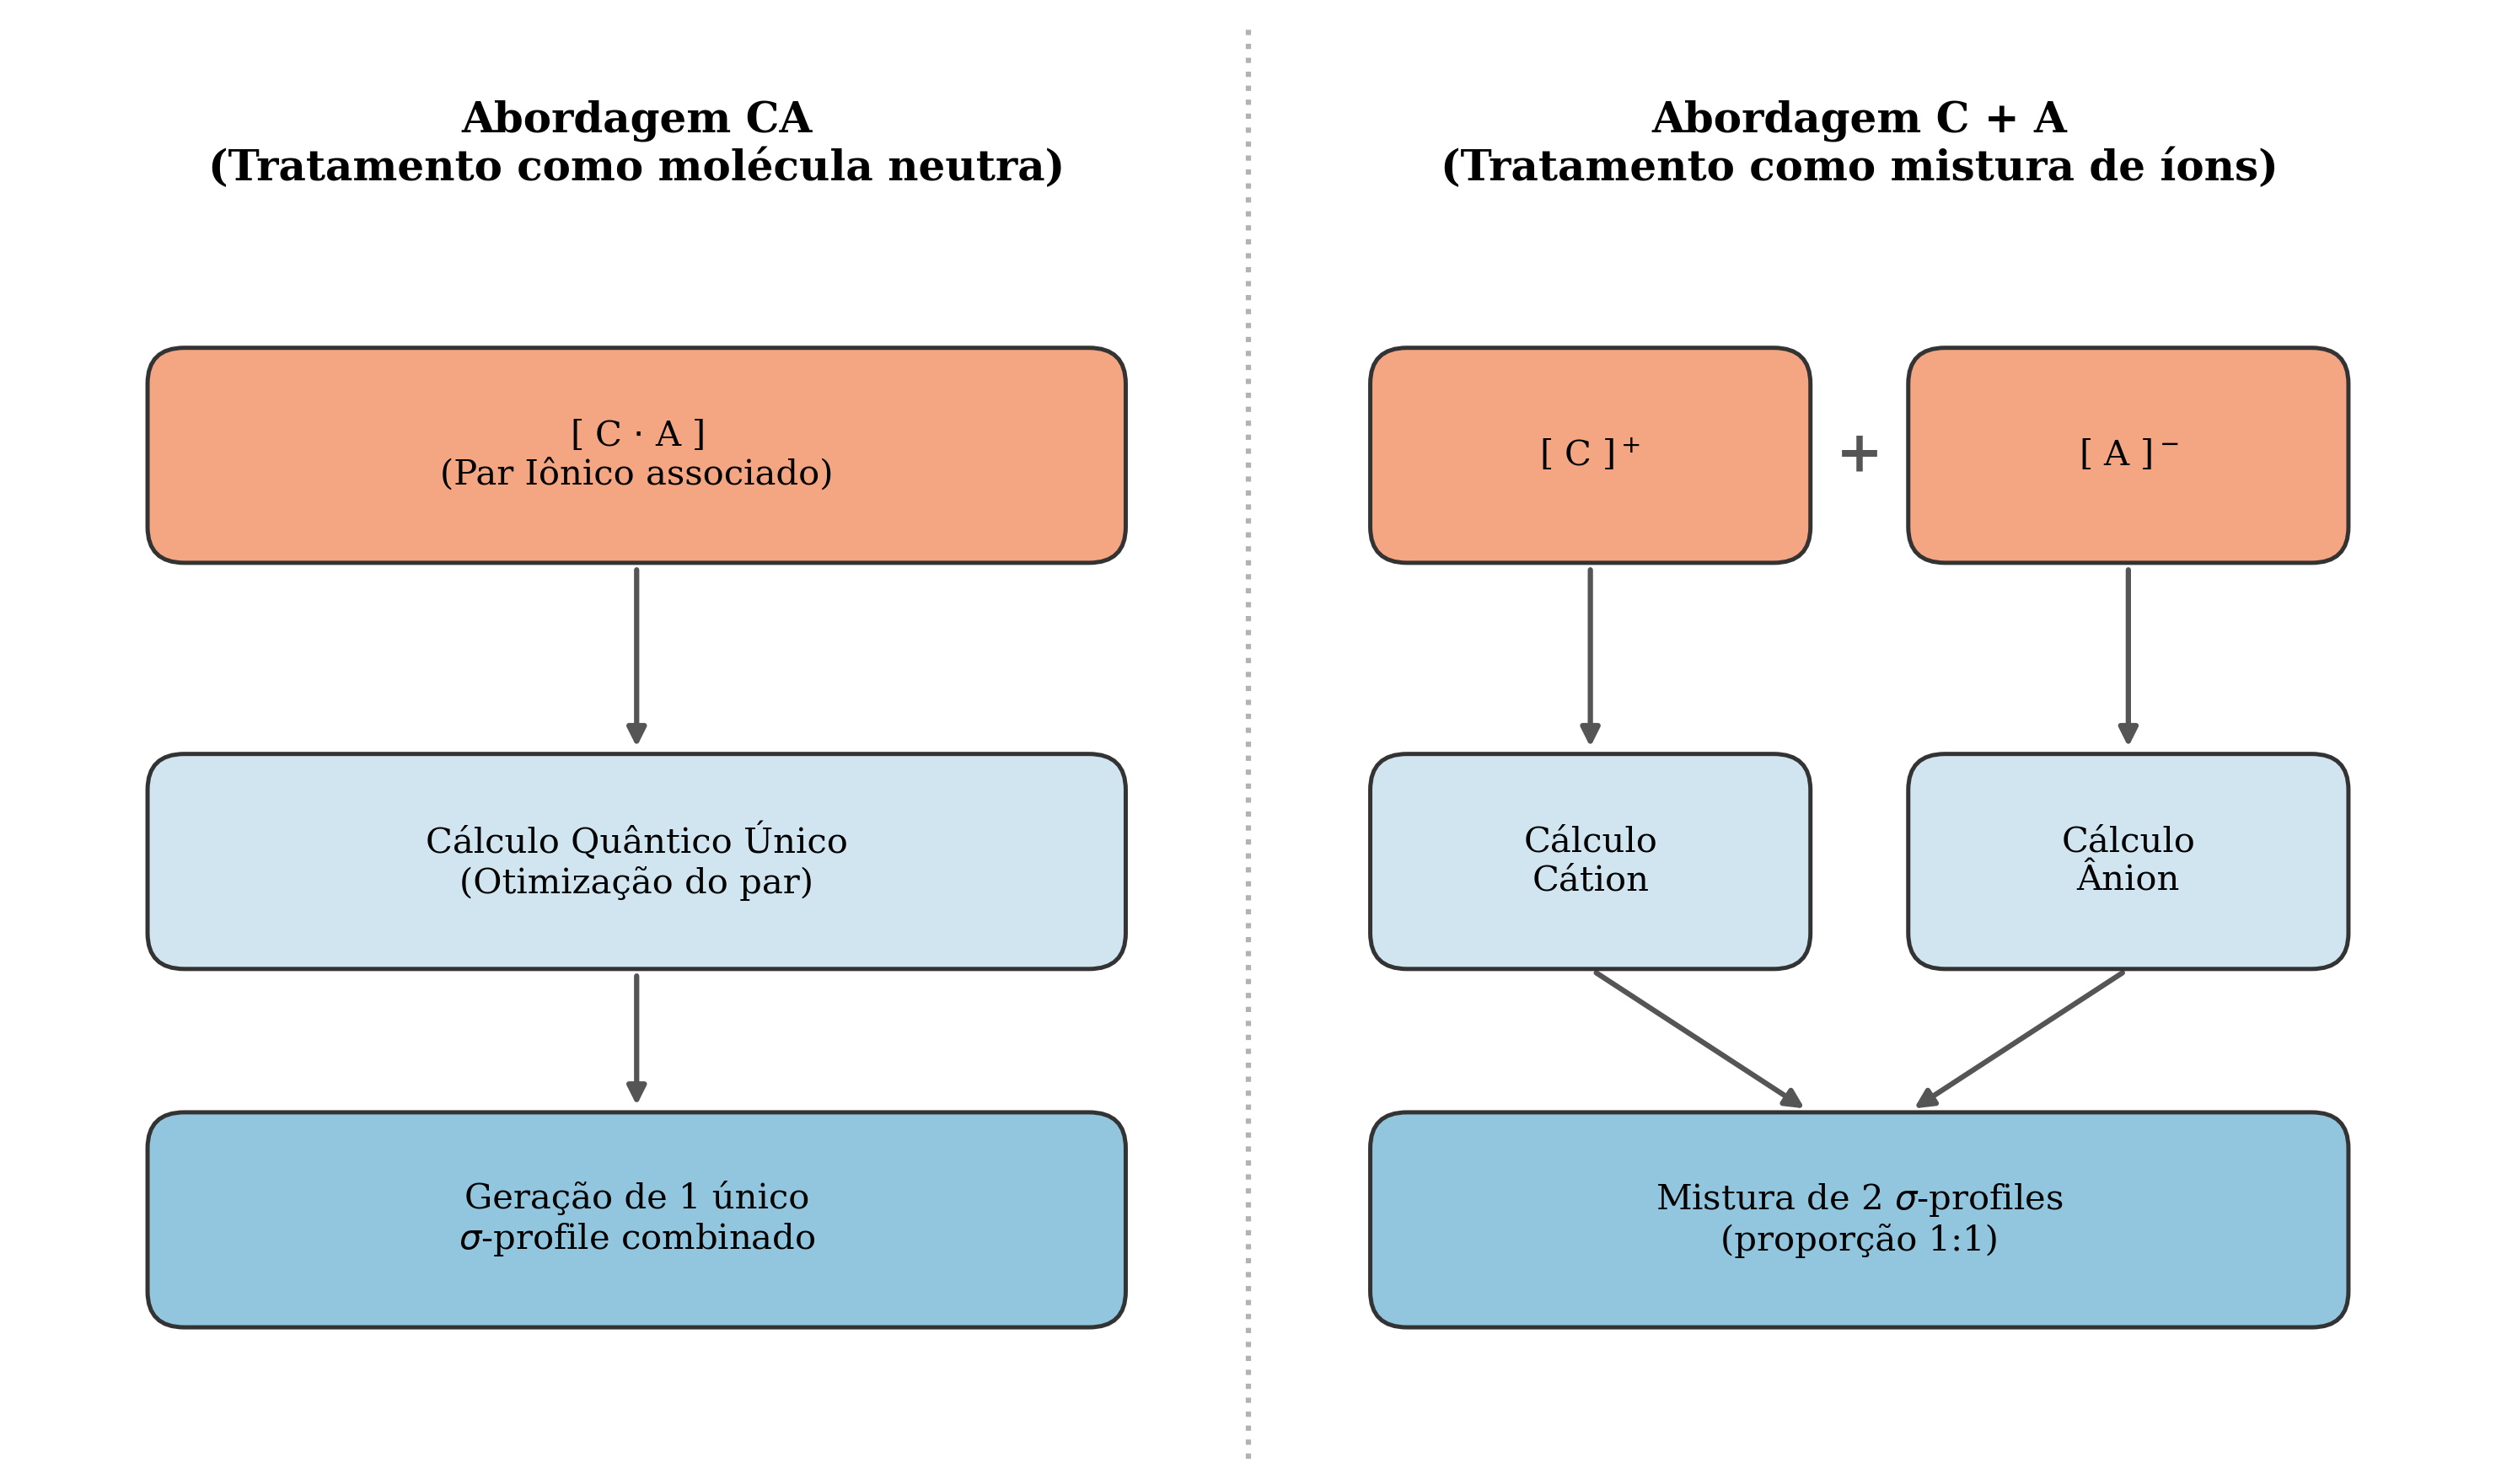
\includegraphics[width=0.7\linewidth]{imagens/fig3_esquema_CA.png}
    \caption{Comparação esquemática entre as abordagens CA (par iônico neutro) e C+A (íons separados), ilustrando a construção dos $\sigma$-profiles em cada caso.}
    \label{fig:CA_C+A}
\end{figure}

Esse precedente da literatura motivou a avaliação inicial da abordagem C+A para os líquidos iônicos próticos deste trabalho. Os cálculos COSMO foram realizados separadamente para os cátions [2-HEA]$^+$ e [DETA]$^+$ e para o ânion hexanoato [Hx]$^-$, e os $\sigma$-profiles combinados conforme a Equação~\ref{eq:sigma_profile_ca}. Essa avaliação, no entanto, revelou uma limitação prática severa: os coeficientes de atividade em diluição infinita calculados a partir dos íons separados assumiram valores fisicamente implausíveis, da ordem de $10^{11}$ a $10^{15}$, muito acima do que se observa para qualquer par soluto-solvente real. Esse resultado indica que, ao separar cátion e ânion em cavidades COSMO independentes, o modelo perde a compensação eletrostática que naturalmente ocorre entre as duas espécies quando associadas, superestimando de forma acentuada a energia de restauração de cada íon isolado.

Diante dessa limitação, adotou-se neste trabalho a abordagem CA (par iônico neutro) para os líquidos iônicos próticos [2-HEA][Hx] e [DETA][Hx] no COSMO-SAC, na mesma linha da estratégia já adotada para o UNIFAC-LL (Seção~\ref{sec:unifacll}). O cálculo COSMO é realizado sobre o par cátion-ânion como uma única entidade neutra, o que produziu coeficientes de atividade com magnitude fisicamente coerente e consistente com o comportamento esperado para líquidos iônicos em solução. Essa escolha diverge do precedente estabelecido por \citeonline{dominguez2014} e \citeonline{xu2022} para líquidos iônicos de imidazólio, o que sugere que a superioridade relativa entre as duas abordagens pode depender da estrutura específica do líquido iônico em questão, e não constitui uma regra geral aplicável a qualquer combinação cátion-ânion. Os detalhes do nível de teoria empregado nos cálculos COSMO de cada par iônico são apresentados no Capítulo~\ref{cap:metodologia}.

\section{O modelo UNIFAC-LL}
\label{sec:unifacll}

O UNIFAC (\textit{UNIversal quasichemical Functional group Activity Coefficients}), proposto por \citeonline{fredenslund1975}, é um modelo de coeficiente de atividade baseado no conceito de contribuição por grupos funcionais. A premissa central é que uma molécula pode ser representada como um conjunto de grupos estruturais (por exemplo, \ce{CH3}, \ce{CH2}, \ce{OH}, \ce{COOH}, \ce{NH2}), e que as interações intermoleculares na mistura podem ser aproximadas pelas interações entre esses grupos, independentemente da molécula à qual pertencem\cite{fredenslund1975}. A variante UNIFAC-LL, parametrizada por \citeonline{magnussen1981} especificamente para a predição de equilíbrio líquido-líquido, é a versão empregada no Capítulo\ref{cap:resultados} deste trabalho como referência comparativa ao COSMO-SAC.

% -----------------------------------------------------------------
% Estrutura do coeficiente de atividade
% -----------------------------------------------------------------

Assim como no COSMO-SAC, o coeficiente de atividade no UNIFAC é expresso como a soma de uma contribuição combinatorial e uma contribuição residual\cite{fredenslund1975}:

\begin{equation}
    \ln \gamma_i = \ln \gamma_i^{comb} + \ln \gamma_i^{res}
    \label{eq:gamma_unifac}
\end{equation}

A contribuição combinatorial é calculada pelo mesmo modelo de Staverman-Guggenheim apresentado na Equação\ref{eq:gamma_combinatorial}, com a diferença de que os parâmetros de volume ($R_k$) e área superficial ($Q_k$) de cada grupo funcional são valores tabelados, obtidos a partir de dados de van der Waals, e não da cavidade COSMO\cite{fredenslund1975}. O volume e a área normalizados de cada molécula são calculados como a soma das contribuições de todos os grupos que a compõem:

\begin{equation}
    r_i = \sum_{k} \nu_k^{(i)} R_k \qquad \text{e} \qquad
    q_i = \sum_{k} \nu_k^{(i)} Q_k
    \label{eq:rq_unifac}
\end{equation}

\noindent em que $\nu_k^{(i)}$ é o número de grupos do tipo $k$ na molécula $i$, e $R_k$ e $Q_k$ são os parâmetros de volume e área do grupo $k$.

% -----------------------------------------------------------------
% Contribuição residual
% -----------------------------------------------------------------

A contribuição residual, por outro lado, difere fundamentalmente da abordagem COSMO-SAC. No UNIFAC, ela é calculada a partir das interações entre pares de grupos funcionais, e não entre segmentos de superfície\cite{fredenslund1975}:

\begin{equation}
    \ln \gamma_i^{res} = \sum_{k} \nu_k^{(i)}
    \left[ \ln \Gamma_k - \ln \Gamma_k^{(i)} \right]
    \label{eq:gamma_res_unifac}
\end{equation}

\noindent em que $\Gamma_k$ é o coeficiente de atividade do grupo $k$ na mistura e $\Gamma_k^{(i)}$ é o coeficiente de atividade do mesmo grupo em uma solução de referência contendo apenas moléculas do tipo $i$. O coeficiente de atividade de grupo é dado por\cite{fredenslund1975}:

\begin{equation}
    \ln \Gamma_k = Q_k \left[
    1 - \ln\!\left(\sum_{m} \Theta_m \Psi_{mk}\right)
    - \sum_{m} \frac{\Theta_m \Psi_{km}}
                    {\displaystyle\sum_{n} \Theta_n \Psi_{nm}}
    \right]
    \label{eq:gamma_grupo}
\end{equation}

\noindent em que $\Theta_m$ é a fração de área superficial do grupo $m$ na mistura e $\Psi_{mn}$ é o parâmetro de interação entre os grupos $m$ e $n$, definido como:

\begin{equation}
    \Psi_{mn} = \exp\!\left(-\frac{a_{mn}}{T}\right)
    \label{eq:psi_unifac}
\end{equation}

Os parâmetros $a_{mn}$ (em unidades de Kelvin) são os parâmetros de interação binários entre grupos, e constituem o elemento central da capacidade preditiva do modelo. Eles são determinados por regressão a partir de dados experimentais de equilíbrio de fases de sistemas conhecidos e organizados em uma matriz de parâmetros de interação, na qual cada entrada corresponde a um par de grupos funcionais\cite{magnussen1981}. Uma vez disponíveis, esses parâmetros permitem predizer o comportamento de qualquer mistura cujas moléculas sejam decomponíveis nos grupos tabelados. A parametrização de \citeonline{magnussen1981} para ELL (UNIFAC-LL) abrange um conjunto de grupos especificamente ajustado à descrição de sistemas com duas fases líquidas, com parâmetros de interação distintos daqueles utilizados nas versões do UNIFAC para equilíbrio líquido-vapor.

% -----------------------------------------------------------------
% Limitações para líquidos iônicos
% -----------------------------------------------------------------

A natureza preditiva do UNIFAC-LL está, portanto, condicionada à disponibilidade de parâmetros de interação para todos os pares de grupos presentes no sistema de interesse. Essa condição impõe uma limitação estrutural quando o modelo é aplicado a sistemas contendo líquidos iônicos. Os cátions e ânions dos LIs podem, em princípio, ser decompostos em grupos funcionais existentes na tabela UNIFAC (por exemplo, \ce{CH2}, \ce{OH}, \ce{NH2}, \ce{COOH}). No entanto, a matriz de Magnussen não contém parâmetros de interação para diversos pares de grupos que surgem quando os grupos representativos dos LIs interagem entre si ou com os demais componentes do sistema\cite{bahadur2015}.

No caso específico dos sistemas estudados neste trabalho, a decomposição dos LIPs [2-HEA][Hx] e [DETA][Hx] em grupos UNIFAC gera pares de interação para os quais os parâmetros $a_{mn}$ são inexistentes na parametrização de Magnussen, como os pares envolvendo grupos \ce{CNH2}/\ce{CCOO} e \ce{CCOO}/\ce{CNH2}. Sem esses parâmetros, o cálculo dos coeficientes de atividade das espécies iônicas seria inviável, o que exige o preenchimento dessa lacuna por meio de um modelo preditivo de aprendizado de máquina, conforme detalhado no Capítulo~\ref{cap:metodologia}. Essa lacuna não é de implementação, mas sim estrutural: decorre do fato de que a matriz de parâmetros foi construída a partir de dados experimentais de sistemas orgânicos convencionais, nos quais líquidos iônicos não estavam presentes\cite{bahadur2015,magnussen1981}, e sua resolução via aprendizado de máquina, em vez de calibração direta, é retomada na discussão das limitações do modelo (Capítulo~\ref{cap:resultados}).

\begin{figure}[H]
    \centering
    \resizebox{\textwidth}{!}{%
    \begin{tikzpicture}[
        group/.style={thick, rounded corners, inner sep=3pt},
        label/.style={font=\footnotesize}
    ]
    
    % ── ETANOL ───────────────────────────────────
    \node[font=\large] at (-2, 5.5) {\textbf{Etanol}};
    
    \node (ch3) at (0, 5) {H$_3$C};
    \node (ch2) at (2, 5) {CH$_2$};
    \node (oh)  at (4, 5) {OH};
    
    \draw[thick] (ch3) -- (ch2) -- (oh);
    
    \node[draw=blue, group, fit=(ch3)] {};
    \node[draw=red, group, fit=(ch2)] {};
    \node[draw=teal, group, fit=(oh)] {};
    
    \node[blue, label] at (0, 6.0) {CH$_3$};
    \node[red, label]  at (2, 6.0) {CH$_2$};
    \node[teal, label] at (4, 6.0) {OH};
    
    % ── [2-HEA][Hx]: PAR IÔNICO NEUTRO COMPLETO ──
    \node[font=\large] at (-2.5, 2.5) {\textbf{[2-HEA][Hx] (par neutro)}};
    
    % Cátion [2-HEA]+
    \node (oh2)  at (0, 2) {HO};
    \node (c2a)  at (2, 2) {CH$_2$};
    \node (nh3)  at (4.2, 2) {NH$_3^+$};
    
    \draw[thick] (oh2) -- (c2a) -- (nh3);
    
    \node[draw=teal, group, fit=(oh2)] {};
    \node[draw=red, group, fit=(c2a)] {};
    \node[draw=purple, group, fit=(nh3)] {};
    
    \node[teal, label]   at (0, 1.0) {OH};
    \node[red, label]    at (2, 1.0) {CH$_2$};
    \node[purple, label] at (4.2, 1.0) {CNH$_2$};
    
    % Interação iônica (par neutro)
    \draw[thick, dotted, gray] (nh3) -- (6.4, 2)
        node[midway, above, font=\footnotesize\itshape, gray] {par iônico};
    
    % Ânion [Hx]- (carboxilato: grupo COO, distinto do éster CCOO dos triglicerídeos)
    \node (coo)  at (6.4, 2) {$^{-}$OOC};
    \node (c3a)  at (8.4, 2) {CH$_2$};
    \node (c3b)  at (10.4, 2) {CH$_2$};
    \node (c3c)  at (12.4, 2) {CH$_2$};
    \node (c3d)  at (14.4, 2) {CH$_2$};
    \node (ch3b) at (16.4, 2) {CH$_3$};
    
    \draw[thick] (coo) -- (c3a) -- (c3b) -- (c3c) -- (c3d) -- (ch3b);
    
    \node[draw=orange, group, fit=(coo)] {};
    \node[draw=red, group, fit=(c3a)] {};
    \node[draw=red, group, fit=(c3b)] {};
    \node[draw=red, group, fit=(c3c)] {};
    \node[draw=red, group, fit=(c3d)] {};
    \node[draw=blue, group, fit=(ch3b)] {};
    
    \node[orange, label] at (6.4, 1.0)  {COO};
    \node[red, label]    at (8.4, 1.0)  {CH$_2$};
    \node[red, label]    at (10.4, 1.0) {CH$_2$};
    \node[red, label]    at (12.4, 1.0) {CH$_2$};
    \node[red, label]    at (14.4, 1.0) {CH$_2$};
    \node[blue, label]   at (16.4, 1.0) {CH$_3$};
    
    \end{tikzpicture}%
    }
    
    \caption{Decomposição em grupos UNIFAC para o etanol
    (1 CH$_3$ + 1 CH$_2$ + 1 OH) e para o par iônico neutro [2-HEA][Hx]
    (cátion: 1 OH + 1 CH$_2$ + 1 CNH$_2$; ânion: 1 COO + 4 CH$_2$ + 1 CH$_3$),
    tratado como uma única espécie neutra pelo modelo. O grupo COO(41)
    do carboxilato aniônico é distinto do grupo éster CCOO(11) presente
    nos triglicerídeos (Tabela~\ref{tab:decomposicao_unifac}), refletindo
    o diferente ambiente químico de cada ligação carbono-oxigênio.}
    \label{fig:unifac_decomposition}
\end{figure}

É essa limitação paramétrica, contrastada com a natureza a priori do COSMO-SAC discutida na Seção~\ref{subsec:cosmo_parametros}, que motiva a comparação sistemática entre os dois modelos neste trabalho, conforme discutido na introdução (Capítulo \ref{introducao}).

\begin{longtable}{p{3.2cm}p{5.4cm}p{5.4cm}}
\caption{Comparação entre os modelos UNIFAC-LL e COSMO-SAC.}
\label{tab:comparacao_modelos} \\
\toprule
\textbf{Característica} & \textbf{UNIFAC-LL} & \textbf{COSMO-SAC} \\
\midrule
\endfirsthead

\multicolumn{3}{c}{\tablename\ \thetable\ -- continuação} \\
\toprule
\textbf{Característica} & \textbf{UNIFAC-LL} & \textbf{COSMO-SAC} \\
\midrule
\endhead

\bottomrule
\endfoot

Natureza preditiva & Empírico, baseado em contribuição de grupos funcionais (FREDENSLUND; JONES; PRAUSNITZ, 1975) & A priori, baseado em propriedades moleculares calculadas por química quântica (LIN; SANDLER, 2002) \\
\addlinespace
Parâmetros necessários & Parâmetros de interação binários entre grupos ($a_{mn}$), ajustados a dados experimentais de mistura (MAGNUSSEN; RASMUSSEN; FREDENSLUND, 1981) & Parâmetros universais ($a_{eff}$, $r_{eff}$, $f_{pol}$, $c_{hb}$, $\sigma_{hb}$, $r_{std}$, $q_{std}$), calibrados uma única vez e válidos para qualquer sistema (LIN; SANDLER, 2002) \\
\addlinespace
Origem da informação molecular & Decomposição da molécula em grupos funcionais tabelados & $\sigma$-profile obtido por cálculo DFT/COSMO da molécula isolada \\
\addlinespace
Contribuição residual & Interação entre pares de grupos funcionais ($\Psi_{mn}$) & Interação entre segmentos de superfície ($\Delta W(\sigma_m,\sigma_n)$) \\
\addlinespace
Tratamento de líquidos iônicos & Lacuna paramétrica original preenchida por modelo de ML (HAYER et al., 2025), já que a matriz de Magnussen carece de pares como CNH2/CCOO (BAHADUR et al., 2015); adota-se o par iônico neutro & Abordagem C+A avaliada e descartada por gerar $\gamma^\infty$ fisicamente implausível ($10^{11}$--$10^{15}$); adota-se o par iônico neutro (mesma estratégia do UNIFAC-LL) \\
\addlinespace
Dependência de dados experimentais da mistura & Sim, para o ajuste dos parâmetros binários & Não, apenas para validação posterior do modelo \\

\end{longtable}